\documentclass[twoside]{book}

% Packages required by doxygen
\usepackage{fixltx2e}
\usepackage{calc}
\usepackage{doxygen}
\usepackage[export]{adjustbox} % also loads graphicx
\usepackage{graphicx}
\usepackage[utf8]{inputenc}
\usepackage{makeidx}
\usepackage{multicol}
\usepackage{multirow}
\PassOptionsToPackage{warn}{textcomp}
\usepackage{textcomp}
\usepackage[nointegrals]{wasysym}
\usepackage[table]{xcolor}

% Font selection
\usepackage[T1]{fontenc}
\usepackage[scaled=.90]{helvet}
\usepackage{courier}
\usepackage{amssymb}
\usepackage{sectsty}
\renewcommand{\familydefault}{\sfdefault}
\allsectionsfont{%
  \fontseries{bc}\selectfont%
  \color{darkgray}%
}
\renewcommand{\DoxyLabelFont}{%
  \fontseries{bc}\selectfont%
  \color{darkgray}%
}
\newcommand{\+}{\discretionary{\mbox{\scriptsize$\hookleftarrow$}}{}{}}

% Page & text layout
\usepackage{geometry}
\geometry{%
  a4paper,%
  top=2.5cm,%
  bottom=2.5cm,%
  left=2.5cm,%
  right=2.5cm%
}
\tolerance=750
\hfuzz=15pt
\hbadness=750
\setlength{\emergencystretch}{15pt}
\setlength{\parindent}{0cm}
\setlength{\parskip}{3ex plus 2ex minus 2ex}
\makeatletter
\renewcommand{\paragraph}{%
  \@startsection{paragraph}{4}{0ex}{-1.0ex}{1.0ex}{%
    \normalfont\normalsize\bfseries\SS@parafont%
  }%
}
\renewcommand{\subparagraph}{%
  \@startsection{subparagraph}{5}{0ex}{-1.0ex}{1.0ex}{%
    \normalfont\normalsize\bfseries\SS@subparafont%
  }%
}
\makeatother

% Headers & footers
\usepackage{fancyhdr}
\pagestyle{fancyplain}
\fancyhead[LE]{\fancyplain{}{\bfseries\thepage}}
\fancyhead[CE]{\fancyplain{}{}}
\fancyhead[RE]{\fancyplain{}{\bfseries\leftmark}}
\fancyhead[LO]{\fancyplain{}{\bfseries\rightmark}}
\fancyhead[CO]{\fancyplain{}{}}
\fancyhead[RO]{\fancyplain{}{\bfseries\thepage}}
\fancyfoot[LE]{\fancyplain{}{}}
\fancyfoot[CE]{\fancyplain{}{}}
\fancyfoot[RE]{\fancyplain{}{\bfseries\scriptsize Generated by Doxygen }}
\fancyfoot[LO]{\fancyplain{}{\bfseries\scriptsize Generated by Doxygen }}
\fancyfoot[CO]{\fancyplain{}{}}
\fancyfoot[RO]{\fancyplain{}{}}
\renewcommand{\footrulewidth}{0.4pt}
\renewcommand{\chaptermark}[1]{%
  \markboth{#1}{}%
}
\renewcommand{\sectionmark}[1]{%
  \markright{\thesection\ #1}%
}

% Indices & bibliography
\usepackage{natbib}
\usepackage[titles]{tocloft}
\setcounter{tocdepth}{3}
\setcounter{secnumdepth}{5}
\makeindex

% Hyperlinks (required, but should be loaded last)
\usepackage{ifpdf}
\ifpdf
  \usepackage[pdftex,pagebackref=true]{hyperref}
\else
  \usepackage[ps2pdf,pagebackref=true]{hyperref}
\fi
\hypersetup{%
  colorlinks=true,%
  linkcolor=blue,%
  citecolor=blue,%
  unicode%
}

% Custom commands
\newcommand{\clearemptydoublepage}{%
  \newpage{\pagestyle{empty}\cleardoublepage}%
}

\usepackage{caption}
\captionsetup{labelsep=space,justification=centering,font={bf},singlelinecheck=off,skip=4pt,position=top}

%===== C O N T E N T S =====

\begin{document}

% Titlepage & ToC
\hypersetup{pageanchor=false,
             bookmarksnumbered=true,
             pdfencoding=unicode
            }
\pagenumbering{alph}
\begin{titlepage}
\vspace*{7cm}
\begin{center}%
{\Large plant.\+io }\\
\vspace*{1cm}
{\large Generated by Doxygen 1.8.13}\\
\end{center}
\end{titlepage}
\clearemptydoublepage
\pagenumbering{roman}
\tableofcontents
\clearemptydoublepage
\pagenumbering{arabic}
\hypersetup{pageanchor=true}

%--- Begin generated contents ---
\chapter{Wireless Plant Monitoring}
\label{index}\hypertarget{index}{}\subsubsection*{Installation and Building for Re-\/motes}


\begin{DoxyEnumerate}
\item Download and extract the \href{https://developer.arm.com/tools-and-software/open-source-software/developer-tools/gnu-toolchain/gnu-rm/downloads}{\tt A\+RM Toolchain} to {\ttfamily $\sim$/.arm}.
\item Clone the Contiki OS to {\ttfamily $\sim$/.contiki} and install submodules\textbackslash{} 
\begin{DoxyCode}
$ git clone https://gitlab.lrz.de/wsnlab/contiki-remote.git ~/.contiki
$ cd ~/.contiki
$ git submodule update --init
\end{DoxyCode}

\item Install Python Serial\textbackslash{} 
\begin{DoxyCode}
$ pip install pyserial --user
\end{DoxyCode}

\item Building the source for Zolertia Re-\/mote and upload it\textbackslash{} 
\begin{DoxyCode}
$ cd src && ./build
\end{DoxyCode}
 
\end{DoxyEnumerate}
\chapter{Hierarchical Index}
\section{Class Hierarchy}
This inheritance list is sorted roughly, but not completely, alphabetically\+:\begin{DoxyCompactList}
\item Q\+Main\+Window\begin{DoxyCompactList}
\item \contentsline{section}{Main\+Window}{\pageref{classMainWindow}}{}
\end{DoxyCompactList}
\end{DoxyCompactList}

\chapter{Class Index}
\section{Class List}
Here are the classes, structs, unions and interfaces with brief descriptions\+:\begin{DoxyCompactList}
\item\contentsline{section}{\hyperlink{classMainWindow}{Main\+Window} \\*The \hyperlink{classMainWindow}{Main\+Window} class }{\pageref{classMainWindow}}{}
\end{DoxyCompactList}

\chapter{File Index}
\section{File List}
Here is a list of all documented files with brief descriptions\+:\begin{DoxyCompactList}
\item\contentsline{section}{gui/\hyperlink{main_8cpp}{main.\+cpp} }{\pageref{main_8cpp}}{}
\item\contentsline{section}{gui/\hyperlink{mainwindow_8cpp}{mainwindow.\+cpp} }{\pageref{mainwindow_8cpp}}{}
\item\contentsline{section}{gui/\hyperlink{mainwindow_8h}{mainwindow.\+h} }{\pageref{mainwindow_8h}}{}
\item\contentsline{section}{src/\hyperlink{mote__sensors_8c}{mote\+\_\+sensors.\+c} }{\pageref{mote__sensors_8c}}{}
\item\contentsline{section}{src/\hyperlink{mote__sensors_8h}{mote\+\_\+sensors.\+h} }{\pageref{mote__sensors_8h}}{}
\item\contentsline{section}{src/\hyperlink{net__packet_8c}{net\+\_\+packet.\+c} }{\pageref{net__packet_8c}}{}
\item\contentsline{section}{src/\hyperlink{net__packet_8h}{net\+\_\+packet.\+h} }{\pageref{net__packet_8h}}{}
\item\contentsline{section}{src/\hyperlink{plantio_8c}{plantio.\+c} }{\pageref{plantio_8c}}{}
\item\contentsline{section}{src/\hyperlink{plantio_8h}{plantio.\+h} }{\pageref{plantio_8h}}{}
\item\contentsline{section}{src/\hyperlink{routing_8c}{routing.\+c} }{\pageref{routing_8c}}{}
\item\contentsline{section}{src/\hyperlink{routing_8h}{routing.\+h} }{\pageref{routing_8h}}{}
\item\contentsline{section}{src/\hyperlink{serial_8c}{serial.\+c} }{\pageref{serial_8c}}{}
\item\contentsline{section}{src/\hyperlink{serial_8h}{serial.\+h} \\*Defines the serial communication between a node and the G\+UI }{\pageref{serial_8h}}{}
\end{DoxyCompactList}

\chapter{Class Documentation}
\hypertarget{classMainWindow}{}\section{Main\+Window Class Reference}
\label{classMainWindow}\index{Main\+Window@{Main\+Window}}


The \hyperlink{classMainWindow}{Main\+Window} class.  




{\ttfamily \#include $<$mainwindow.\+h$>$}



Inheritance diagram for Main\+Window\+:\nopagebreak
\begin{figure}[H]
\begin{center}
\leavevmode
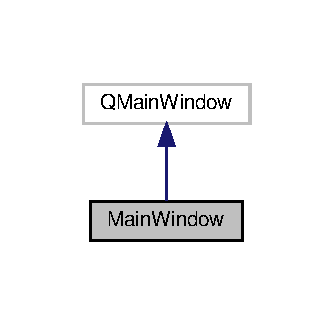
\includegraphics[width=160pt]{classMainWindow__inherit__graph}
\end{center}
\end{figure}


Collaboration diagram for Main\+Window\+:\nopagebreak
\begin{figure}[H]
\begin{center}
\leavevmode
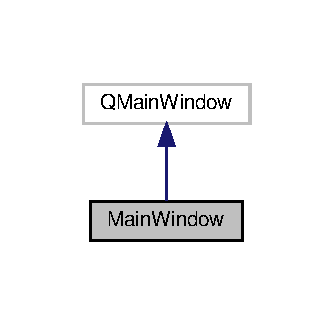
\includegraphics[width=160pt]{classMainWindow__coll__graph}
\end{center}
\end{figure}
\subsection*{Public Member Functions}
\begin{DoxyCompactItemize}
\item 
\mbox{\Hypertarget{classMainWindow_a996c5a2b6f77944776856f08ec30858d}\label{classMainWindow_a996c5a2b6f77944776856f08ec30858d}} 
\hyperlink{classMainWindow_a996c5a2b6f77944776856f08ec30858d}{Main\+Window} (Q\+Widget $\ast$parent=nullptr)
\begin{DoxyCompactList}\small\item\em Main Window setup function. Scans usb ports for motes on startup. Paints text\+Edit background black and text color white for an authentic console experience. \end{DoxyCompactList}\end{DoxyCompactItemize}
\subsection*{Protected Slots}
\begin{DoxyCompactItemize}
\item 
\mbox{\Hypertarget{classMainWindow_a0ed54c0c9e6d0206e716402ade3994ee}\label{classMainWindow_a0ed54c0c9e6d0206e716402ade3994ee}} 
void \hyperlink{classMainWindow_a0ed54c0c9e6d0206e716402ade3994ee}{resend2selection} ()
\begin{DoxyCompactList}\small\item\em Function for handling the retransmissions of unacknowledged requests. After three tries this function recognizes that one or more routes have become invalid and thus a new network exploration is triggered. \end{DoxyCompactList}\item 
\mbox{\Hypertarget{classMainWindow_aa4a61b706dc1ac7eafed167da9fb6cc3}\label{classMainWindow_aa4a61b706dc1ac7eafed167da9fb6cc3}} 
void \hyperlink{classMainWindow_aa4a61b706dc1ac7eafed167da9fb6cc3}{receive} ()
\begin{DoxyCompactList}\small\item\em Function for handling serial messages from the mote. L\+T/\+GT operators $<$$>$ denote important data and are simultaneously used as acknowledgements. Requests from gui that natively don\textquotesingle{}t solicit reply messages return an explicit A\+CK packet with the $<$$>$ format. This gives us consistant and reliable acknowledgements. \end{DoxyCompactList}\item 
\mbox{\Hypertarget{classMainWindow_aaaaabf5c6516ffee58d65f5fdf786c44}\label{classMainWindow_aaaaabf5c6516ffee58d65f5fdf786c44}} 
void \hyperlink{classMainWindow_aaaaabf5c6516ffee58d65f5fdf786c44}{enable\+Button} ()
\begin{DoxyCompactList}\small\item\em Function for enabling the exploration push\+Button after a timeout. Gets called in \hyperlink{classMainWindow_a6de134a18b08532696095fad75d8b9e3}{on\+\_\+push\+Button\+\_\+\+Explore\+\_\+clicked()}. \end{DoxyCompactList}\item 
\mbox{\Hypertarget{classMainWindow_a716f3b40c6e743d44cfcf9252b2a1934}\label{classMainWindow_a716f3b40c6e743d44cfcf9252b2a1934}} 
void \hyperlink{classMainWindow_a716f3b40c6e743d44cfcf9252b2a1934}{on\+\_\+push\+Button\+\_\+\+Open\+\_\+clicked} ()
\begin{DoxyCompactList}\small\item\em Opening the selected U\+SB port. \end{DoxyCompactList}\item 
\mbox{\Hypertarget{classMainWindow_a7646bc6193d4ab29f4871e7ddb7d320a}\label{classMainWindow_a7646bc6193d4ab29f4871e7ddb7d320a}} 
void \hyperlink{classMainWindow_a7646bc6193d4ab29f4871e7ddb7d320a}{on\+\_\+push\+Button\+\_\+\+Close\+\_\+clicked} ()
\begin{DoxyCompactList}\small\item\em Closing the currently open U\+SB port. \end{DoxyCompactList}\item 
\mbox{\Hypertarget{classMainWindow_ab246b4bb1b03c40cf1282e968486aae5}\label{classMainWindow_ab246b4bb1b03c40cf1282e968486aae5}} 
void \hyperlink{classMainWindow_ab246b4bb1b03c40cf1282e968486aae5}{on\+\_\+push\+Button\+\_\+\+Reload\+\_\+clicked} ()
\begin{DoxyCompactList}\small\item\em Function for reloading/refreshing the available ports. \end{DoxyCompactList}\item 
\mbox{\Hypertarget{classMainWindow_a6de134a18b08532696095fad75d8b9e3}\label{classMainWindow_a6de134a18b08532696095fad75d8b9e3}} 
void \hyperlink{classMainWindow_a6de134a18b08532696095fad75d8b9e3}{on\+\_\+push\+Button\+\_\+\+Explore\+\_\+clicked} ()
\begin{DoxyCompactList}\small\item\em Initialize the network exploration. \end{DoxyCompactList}\item 
\mbox{\Hypertarget{classMainWindow_a30b56d6ecaaabe106f51dc385d64e38b}\label{classMainWindow_a30b56d6ecaaabe106f51dc385d64e38b}} 
void \hyperlink{classMainWindow_a30b56d6ecaaabe106f51dc385d64e38b}{on\+\_\+push\+Button\+\_\+\+Zoom\+In\+\_\+clicked} ()
\begin{DoxyCompactList}\small\item\em Zoom in the netowork graph. \end{DoxyCompactList}\item 
\mbox{\Hypertarget{classMainWindow_a803d415d83e648d1c040d4474a978f28}\label{classMainWindow_a803d415d83e648d1c040d4474a978f28}} 
void \hyperlink{classMainWindow_a803d415d83e648d1c040d4474a978f28}{on\+\_\+push\+Button\+\_\+\+Zoom\+Out\+\_\+clicked} ()
\begin{DoxyCompactList}\small\item\em Zoom out the network graph. \end{DoxyCompactList}\item 
\mbox{\Hypertarget{classMainWindow_ab391669c647ea75c64e2e1258323d286}\label{classMainWindow_ab391669c647ea75c64e2e1258323d286}} 
void \hyperlink{classMainWindow_ab391669c647ea75c64e2e1258323d286}{on\+\_\+push\+Button\+\_\+\+Set\+Max\+\_\+clicked} ()
\begin{DoxyCompactList}\small\item\em Set the maximum amount of motes in the network. This helps scaling the A\+CK timeout and network visualization. \end{DoxyCompactList}\item 
\mbox{\Hypertarget{classMainWindow_a362f1eff4b76dfa1761db912e99e7083}\label{classMainWindow_a362f1eff4b76dfa1761db912e99e7083}} 
void \hyperlink{classMainWindow_a362f1eff4b76dfa1761db912e99e7083}{on\+\_\+push\+Button\+\_\+\+Refresh\+\_\+\+Tab2\+\_\+clicked} ()
\begin{DoxyCompactList}\small\item\em Refreshes the list\+Widget items on tab 2. \end{DoxyCompactList}\item 
\mbox{\Hypertarget{classMainWindow_aa391a38cfddba913c5a3a3a96e7dc00f}\label{classMainWindow_aa391a38cfddba913c5a3a3a96e7dc00f}} 
void \hyperlink{classMainWindow_aa391a38cfddba913c5a3a3a96e7dc00f}{on\+\_\+push\+Button\+\_\+\+Select\+All\+\_\+\+Tab2\+\_\+clicked} ()
\begin{DoxyCompactList}\small\item\em Selects all list\+Widget items on tab 2. \end{DoxyCompactList}\item 
\mbox{\Hypertarget{classMainWindow_a96ce66930f135a8788b1b77d22e404e6}\label{classMainWindow_a96ce66930f135a8788b1b77d22e404e6}} 
void \hyperlink{classMainWindow_a96ce66930f135a8788b1b77d22e404e6}{on\+\_\+push\+Button\+\_\+\+Unselect\+All\+\_\+\+Tab2\+\_\+clicked} ()
\begin{DoxyCompactList}\small\item\em Unselects all list\+Widget items on tab 2. \end{DoxyCompactList}\item 
\mbox{\Hypertarget{classMainWindow_a886cb1ed2510a7fc3de35874eab50a19}\label{classMainWindow_a886cb1ed2510a7fc3de35874eab50a19}} 
void \hyperlink{classMainWindow_a886cb1ed2510a7fc3de35874eab50a19}{on\+\_\+push\+Button\+\_\+\+Refresh\+\_\+\+Tab3\+\_\+clicked} ()
\begin{DoxyCompactList}\small\item\em Refreshes the list\+Widget items on tab 3. \end{DoxyCompactList}\item 
\mbox{\Hypertarget{classMainWindow_a5799237eb83637aa8aca620f2043da5a}\label{classMainWindow_a5799237eb83637aa8aca620f2043da5a}} 
void \hyperlink{classMainWindow_a5799237eb83637aa8aca620f2043da5a}{on\+\_\+push\+Button\+\_\+\+Select\+All\+\_\+\+Tab3\+\_\+clicked} ()
\begin{DoxyCompactList}\small\item\em Selects all list\+Widget items on tab 3. \end{DoxyCompactList}\item 
\mbox{\Hypertarget{classMainWindow_ae9a30c4c371e2c2ce6f7354875368351}\label{classMainWindow_ae9a30c4c371e2c2ce6f7354875368351}} 
void \hyperlink{classMainWindow_ae9a30c4c371e2c2ce6f7354875368351}{on\+\_\+push\+Button\+\_\+\+Unselect\+All\+\_\+\+Tab3\+\_\+clicked} ()
\begin{DoxyCompactList}\small\item\em Unselects all list\+Widget items on tab 3. \end{DoxyCompactList}\item 
\mbox{\Hypertarget{classMainWindow_ae63340fe5e458e1160709c81a1ca3956}\label{classMainWindow_ae63340fe5e458e1160709c81a1ca3956}} 
void \hyperlink{classMainWindow_ae63340fe5e458e1160709c81a1ca3956}{on\+\_\+push\+Button\+\_\+\+Send\+Temp\+\_\+clicked} ()
\begin{DoxyCompactList}\small\item\em Configure temperature thresholds. \end{DoxyCompactList}\item 
\mbox{\Hypertarget{classMainWindow_a54f3e0176f218037a3901e3c24a93338}\label{classMainWindow_a54f3e0176f218037a3901e3c24a93338}} 
void \hyperlink{classMainWindow_a54f3e0176f218037a3901e3c24a93338}{on\+\_\+push\+Button\+\_\+\+Send\+Hum\+\_\+clicked} ()
\begin{DoxyCompactList}\small\item\em Configure humidity thresholds. \end{DoxyCompactList}\item 
\mbox{\Hypertarget{classMainWindow_a083c03ea7e282b677e5d2d9108ccd5e5}\label{classMainWindow_a083c03ea7e282b677e5d2d9108ccd5e5}} 
void \hyperlink{classMainWindow_a083c03ea7e282b677e5d2d9108ccd5e5}{on\+\_\+push\+Button\+\_\+\+Send\+Light\+\_\+clicked} ()
\begin{DoxyCompactList}\small\item\em Configure light thresholds. \end{DoxyCompactList}\item 
\mbox{\Hypertarget{classMainWindow_abb4b4fb07a781d7e69e97be136406895}\label{classMainWindow_abb4b4fb07a781d7e69e97be136406895}} 
void \hyperlink{classMainWindow_abb4b4fb07a781d7e69e97be136406895}{on\+\_\+push\+Button\+\_\+\+Send\+All\+\_\+clicked} ()
\begin{DoxyCompactList}\small\item\em Configure all thresholds. \end{DoxyCompactList}\item 
\mbox{\Hypertarget{classMainWindow_a286fcb906abc360a3b51626bdc549122}\label{classMainWindow_a286fcb906abc360a3b51626bdc549122}} 
void \hyperlink{classMainWindow_a286fcb906abc360a3b51626bdc549122}{on\+\_\+push\+Button\+\_\+\+Get\+All\+\_\+clicked} ()
\begin{DoxyCompactList}\small\item\em Fetch all thresholds. \end{DoxyCompactList}\item 
\mbox{\Hypertarget{classMainWindow_aeceef6b26d35f48752f5c95f529b4166}\label{classMainWindow_aeceef6b26d35f48752f5c95f529b4166}} 
void \hyperlink{classMainWindow_aeceef6b26d35f48752f5c95f529b4166}{on\+\_\+push\+Button\+\_\+\+Center\+\_\+clicked} ()
\begin{DoxyCompactList}\small\item\em Center and rescale the network topology graph with a small border for improved aesthetics. \end{DoxyCompactList}\item 
\mbox{\Hypertarget{classMainWindow_ab753cd6f5aa04ec2716b23da14a17c3a}\label{classMainWindow_ab753cd6f5aa04ec2716b23da14a17c3a}} 
void \hyperlink{classMainWindow_ab753cd6f5aa04ec2716b23da14a17c3a}{on\+\_\+push\+Button\+\_\+\+Clear\+\_\+clicked} ()
\begin{DoxyCompactList}\small\item\em Clear console. \end{DoxyCompactList}\item 
\mbox{\Hypertarget{classMainWindow_a19288f19ebf126204a575b7a71f73ef0}\label{classMainWindow_a19288f19ebf126204a575b7a71f73ef0}} 
void \hyperlink{classMainWindow_a19288f19ebf126204a575b7a71f73ef0}{on\+\_\+push\+Button\+\_\+\+Get\+Sensor\+Data\+\_\+clicked} ()
\begin{DoxyCompactList}\small\item\em Function for initializing the sensor plots and requesting the sensor data from the selection. \end{DoxyCompactList}\item 
\mbox{\Hypertarget{classMainWindow_a4c69446fb6a0d787f8901333eec2ce3a}\label{classMainWindow_a4c69446fb6a0d787f8901333eec2ce3a}} 
void \hyperlink{classMainWindow_a4c69446fb6a0d787f8901333eec2ce3a}{on\+\_\+push\+Button\+\_\+\+Get\+Routing\+Table\+\_\+clicked} ()
\begin{DoxyCompactList}\small\item\em Get routing tables. \end{DoxyCompactList}\item 
\mbox{\Hypertarget{classMainWindow_a30ae116f22bf182d4aec0fe7776e6144}\label{classMainWindow_a30ae116f22bf182d4aec0fe7776e6144}} 
void \hyperlink{classMainWindow_a30ae116f22bf182d4aec0fe7776e6144}{on\+\_\+push\+Button\+\_\+\+L\+E\+D\+\_\+clicked} ()
\begin{DoxyCompactList}\small\item\em Set L\+ED colors. \end{DoxyCompactList}\end{DoxyCompactItemize}
\subsection*{Protected Member Functions}
\begin{DoxyCompactItemize}
\item 
void \hyperlink{classMainWindow_af4ca5d0d3d18ddcb7d54b6596bbf4797}{change\+Event} (Q\+Event $\ast$e)
\begin{DoxyCompactList}\small\item\em change\+Event \end{DoxyCompactList}\item 
\mbox{\Hypertarget{classMainWindow_a3148593d5ab6ac6007967a4c43e28c16}\label{classMainWindow_a3148593d5ab6ac6007967a4c43e28c16}} 
void \hyperlink{classMainWindow_a3148593d5ab6ac6007967a4c43e28c16}{reset\+\_\+graph} ()
\begin{DoxyCompactList}\small\item\em Reset all arrays associated with the topology visualization graph. \end{DoxyCompactList}\item 
void \hyperlink{classMainWindow_aa74278d87740ad86c6db91f071f7fd19}{create\+\_\+graph} (Q\+String\+List list)
\begin{DoxyCompactList}\small\item\em Function for creating visualization of the sensor network topology. Every time a route is received this function is called to plot the route. \end{DoxyCompactList}\item 
void \hyperlink{classMainWindow_af2cff5831eb2f2d562a070183b0f24af}{send2port} (Q\+String msg)
\begin{DoxyCompactList}\small\item\em Send serial commands to the connected mote. \end{DoxyCompactList}\item 
void \hyperlink{classMainWindow_ad87cfafc21d51c74902c8eb99b7fd90f}{print} (Q\+String msg)
\begin{DoxyCompactList}\small\item\em Helper function for outputting messages to the console. \end{DoxyCompactList}\item 
void \hyperlink{classMainWindow_aef3981280b4d81ab4b880e435a992ebd}{plot} (int type, Q\+String\+List data, Q\+String id)
\begin{DoxyCompactList}\small\item\em Function for plotting received sensor data. \end{DoxyCompactList}\item 
void \hyperlink{classMainWindow_ab053f15eaeb520f97732c5745a11bc9e}{send2selection} (Q\+List\+Widget $\ast$list\+Widget, Q\+String request\+Type)
\begin{DoxyCompactList}\small\item\em Function for sending a certain serial request to all selected motes from the corresponding list\+Widget. \end{DoxyCompactList}\end{DoxyCompactItemize}
\subsection*{Protected Attributes}
\begin{DoxyCompactItemize}
\item 
\mbox{\Hypertarget{classMainWindow_a35466a70ed47252a0191168126a352a5}\label{classMainWindow_a35466a70ed47252a0191168126a352a5}} 
Ui\+::\+Main\+Window $\ast$ {\bfseries ui}
\item 
\mbox{\Hypertarget{classMainWindow_a7ecc506a570874a14ec96b4a5a542a80}\label{classMainWindow_a7ecc506a570874a14ec96b4a5a542a80}} 
Qext\+Serial\+Port {\bfseries port}
\item 
\mbox{\Hypertarget{classMainWindow_ad44cc683935445cf008ca045ad90b322}\label{classMainWindow_ad44cc683935445cf008ca045ad90b322}} 
Q\+Message\+Box {\bfseries error}
\item 
\mbox{\Hypertarget{classMainWindow_a0b0049181ace3b8e132cb1ca1c93c871}\label{classMainWindow_a0b0049181ace3b8e132cb1ca1c93c871}} 
Q\+Graphics\+Scene $\ast$ {\bfseries m\+Scene}
\end{DoxyCompactItemize}


\subsection{Detailed Description}
The \hyperlink{classMainWindow}{Main\+Window} class. 

\subsection{Member Function Documentation}
\mbox{\Hypertarget{classMainWindow_af4ca5d0d3d18ddcb7d54b6596bbf4797}\label{classMainWindow_af4ca5d0d3d18ddcb7d54b6596bbf4797}} 
\index{Main\+Window@{Main\+Window}!change\+Event@{change\+Event}}
\index{change\+Event@{change\+Event}!Main\+Window@{Main\+Window}}
\subsubsection{\texorpdfstring{change\+Event()}{changeEvent()}}
{\footnotesize\ttfamily void Main\+Window\+::change\+Event (\begin{DoxyParamCaption}\item[{Q\+Event $\ast$}]{e }\end{DoxyParamCaption})\hspace{0.3cm}{\ttfamily [protected]}}



change\+Event 


\begin{DoxyParams}{Parameters}
{\em e} & \\
\hline
\end{DoxyParams}
\mbox{\Hypertarget{classMainWindow_aa74278d87740ad86c6db91f071f7fd19}\label{classMainWindow_aa74278d87740ad86c6db91f071f7fd19}} 
\index{Main\+Window@{Main\+Window}!create\+\_\+graph@{create\+\_\+graph}}
\index{create\+\_\+graph@{create\+\_\+graph}!Main\+Window@{Main\+Window}}
\subsubsection{\texorpdfstring{create\+\_\+graph()}{create\_graph()}}
{\footnotesize\ttfamily void Main\+Window\+::create\+\_\+graph (\begin{DoxyParamCaption}\item[{Q\+String\+List}]{list }\end{DoxyParamCaption})\hspace{0.3cm}{\ttfamily [protected]}}



Function for creating visualization of the sensor network topology. Every time a route is received this function is called to plot the route. 


\begin{DoxyParams}{Parameters}
{\em Input\+List} & The optimal route from the respective mote to the gui \\
\hline
\end{DoxyParams}
\mbox{\Hypertarget{classMainWindow_aef3981280b4d81ab4b880e435a992ebd}\label{classMainWindow_aef3981280b4d81ab4b880e435a992ebd}} 
\index{Main\+Window@{Main\+Window}!plot@{plot}}
\index{plot@{plot}!Main\+Window@{Main\+Window}}
\subsubsection{\texorpdfstring{plot()}{plot()}}
{\footnotesize\ttfamily void Main\+Window\+::plot (\begin{DoxyParamCaption}\item[{int}]{type,  }\item[{Q\+String\+List}]{data,  }\item[{Q\+String}]{id }\end{DoxyParamCaption})\hspace{0.3cm}{\ttfamily [protected]}}



Function for plotting received sensor data. 


\begin{DoxyParams}{Parameters}
{\em type} & Type of sensor data\+: 1 = Temperature, 2 = Humidity, 3 = Light \\
\hline
{\em data} & Sensor data to be plotted \\
\hline
{\em id} & Associated mote id \\
\hline
\end{DoxyParams}
\mbox{\Hypertarget{classMainWindow_ad87cfafc21d51c74902c8eb99b7fd90f}\label{classMainWindow_ad87cfafc21d51c74902c8eb99b7fd90f}} 
\index{Main\+Window@{Main\+Window}!print@{print}}
\index{print@{print}!Main\+Window@{Main\+Window}}
\subsubsection{\texorpdfstring{print()}{print()}}
{\footnotesize\ttfamily void Main\+Window\+::print (\begin{DoxyParamCaption}\item[{Q\+String}]{msg }\end{DoxyParamCaption})\hspace{0.3cm}{\ttfamily [protected]}}



Helper function for outputting messages to the console. 


\begin{DoxyParams}{Parameters}
{\em msg} & Message to be printed. \\
\hline
\end{DoxyParams}
\mbox{\Hypertarget{classMainWindow_af2cff5831eb2f2d562a070183b0f24af}\label{classMainWindow_af2cff5831eb2f2d562a070183b0f24af}} 
\index{Main\+Window@{Main\+Window}!send2port@{send2port}}
\index{send2port@{send2port}!Main\+Window@{Main\+Window}}
\subsubsection{\texorpdfstring{send2port()}{send2port()}}
{\footnotesize\ttfamily void Main\+Window\+::send2port (\begin{DoxyParamCaption}\item[{Q\+String}]{msg }\end{DoxyParamCaption})\hspace{0.3cm}{\ttfamily [protected]}}



Send serial commands to the connected mote. 


\begin{DoxyParams}{Parameters}
{\em input} & The command that should be sent over serial communication. \\
\hline
\end{DoxyParams}
\mbox{\Hypertarget{classMainWindow_ab053f15eaeb520f97732c5745a11bc9e}\label{classMainWindow_ab053f15eaeb520f97732c5745a11bc9e}} 
\index{Main\+Window@{Main\+Window}!send2selection@{send2selection}}
\index{send2selection@{send2selection}!Main\+Window@{Main\+Window}}
\subsubsection{\texorpdfstring{send2selection()}{send2selection()}}
{\footnotesize\ttfamily void Main\+Window\+::send2selection (\begin{DoxyParamCaption}\item[{Q\+List\+Widget $\ast$}]{list\+Widget,  }\item[{Q\+String}]{request\+Type }\end{DoxyParamCaption})\hspace{0.3cm}{\ttfamily [protected]}}



Function for sending a certain serial request to all selected motes from the corresponding list\+Widget. 


\begin{DoxyParams}{Parameters}
{\em list\+Widget} & The list\+Widget where the id selection is extracted from \\
\hline
{\em request\+Type} & The type of serial communication request that should be sent to all selected motes \\
\hline
\end{DoxyParams}


The documentation for this class was generated from the following files\+:\begin{DoxyCompactItemize}
\item 
gui/\hyperlink{mainwindow_8h}{mainwindow.\+h}\item 
gui/\hyperlink{mainwindow_8cpp}{mainwindow.\+cpp}\end{DoxyCompactItemize}

\chapter{File Documentation}
\hypertarget{main_8cpp}{}\section{gui/main.cpp File Reference}
\label{main_8cpp}\index{gui/main.\+cpp@{gui/main.\+cpp}}
{\ttfamily \#include $<$Q\+Application$>$}\newline
{\ttfamily \#include \char`\"{}mainwindow.\+h\char`\"{}}\newline
Include dependency graph for main.\+cpp\+:
\nopagebreak
\begin{figure}[H]
\begin{center}
\leavevmode
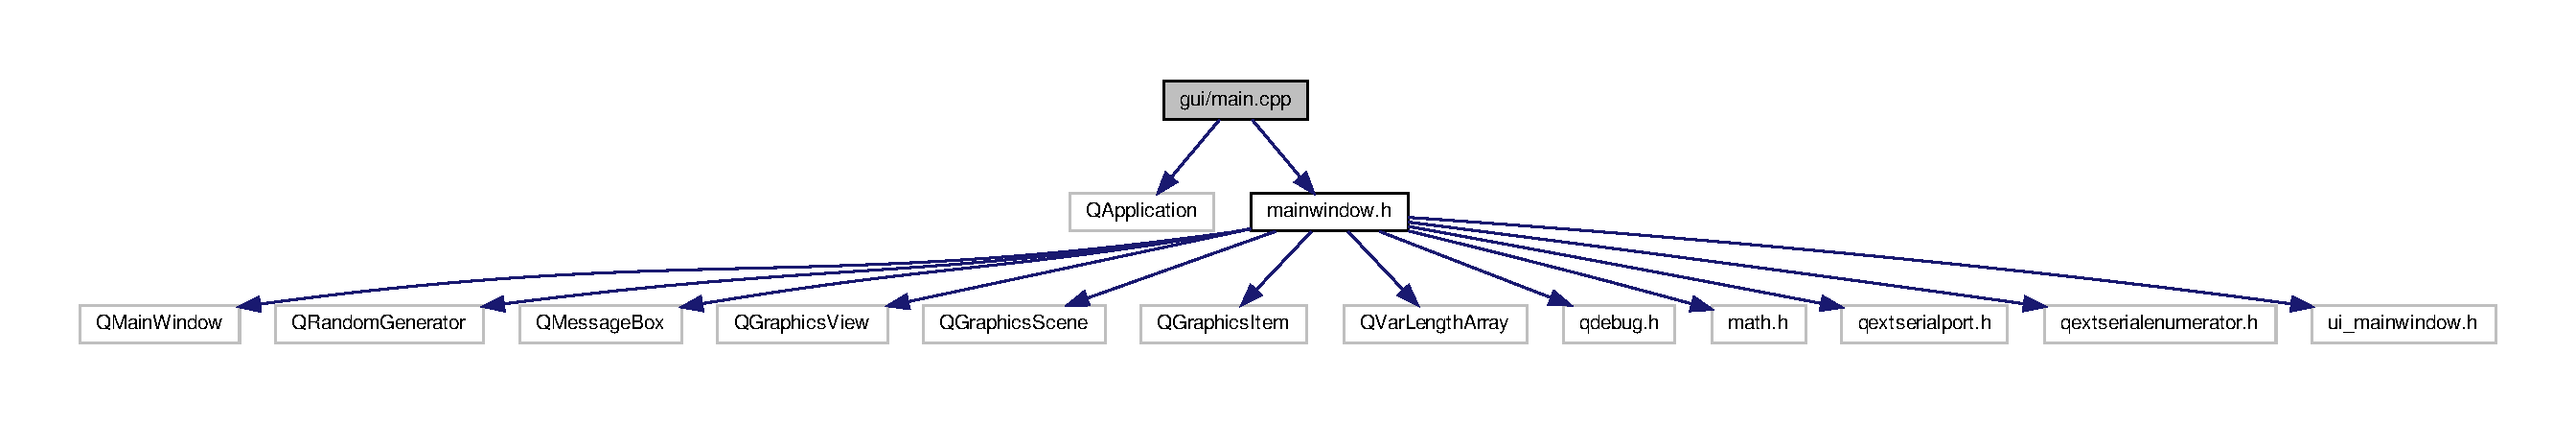
\includegraphics[width=350pt]{main_8cpp__incl}
\end{center}
\end{figure}
\subsection*{Functions}
\begin{DoxyCompactItemize}
\item 
int \hyperlink{main_8cpp_a0ddf1224851353fc92bfbff6f499fa97}{main} (int argc, char $\ast$argv\mbox{[}$\,$\mbox{]})
\begin{DoxyCompactList}\small\item\em main function, initializes the application window. \end{DoxyCompactList}\end{DoxyCompactItemize}


\subsection{Detailed Description}
\begin{DoxyAuthor}{Author}
Patrick Willner (\href{mailto:patrick.willner@tum.de}{\tt patrick.\+willner@tum.\+de}), Andreas Koliopoulos (\href{mailto:ga96leh@mytum.de}{\tt ga96leh@mytum.\+de}), Alexander Schmaus (\href{mailto:ga96fin@mytum.de}{\tt ga96fin@mytum.\+de}) 
\end{DoxyAuthor}
\begin{DoxyVersion}{Version}
1.\+0 
\end{DoxyVersion}
\begin{DoxyDate}{Date}
2019-\/12-\/12
\end{DoxyDate}
\begin{DoxyCopyright}{Copyright}
Copyright (c) 2019 
\end{DoxyCopyright}


\subsection{Function Documentation}
\mbox{\Hypertarget{main_8cpp_a0ddf1224851353fc92bfbff6f499fa97}\label{main_8cpp_a0ddf1224851353fc92bfbff6f499fa97}} 
\index{main.\+cpp@{main.\+cpp}!main@{main}}
\index{main@{main}!main.\+cpp@{main.\+cpp}}
\subsubsection{\texorpdfstring{main()}{main()}}
{\footnotesize\ttfamily int main (\begin{DoxyParamCaption}\item[{int}]{argc,  }\item[{char $\ast$}]{argv\mbox{[}$\,$\mbox{]} }\end{DoxyParamCaption})}



main function, initializes the application window. 


\begin{DoxyParams}{Parameters}
{\em argc} & \\
\hline
{\em argv} & \\
\hline
\end{DoxyParams}
\begin{DoxyReturn}{Returns}

\end{DoxyReturn}

\hypertarget{mainwindow_8cpp}{}\section{gui/mainwindow.cpp File Reference}
\label{mainwindow_8cpp}\index{gui/mainwindow.\+cpp@{gui/mainwindow.\+cpp}}
{\ttfamily \#include \char`\"{}mainwindow.\+h\char`\"{}}\newline
Include dependency graph for mainwindow.\+cpp\+:
\nopagebreak
\begin{figure}[H]
\begin{center}
\leavevmode
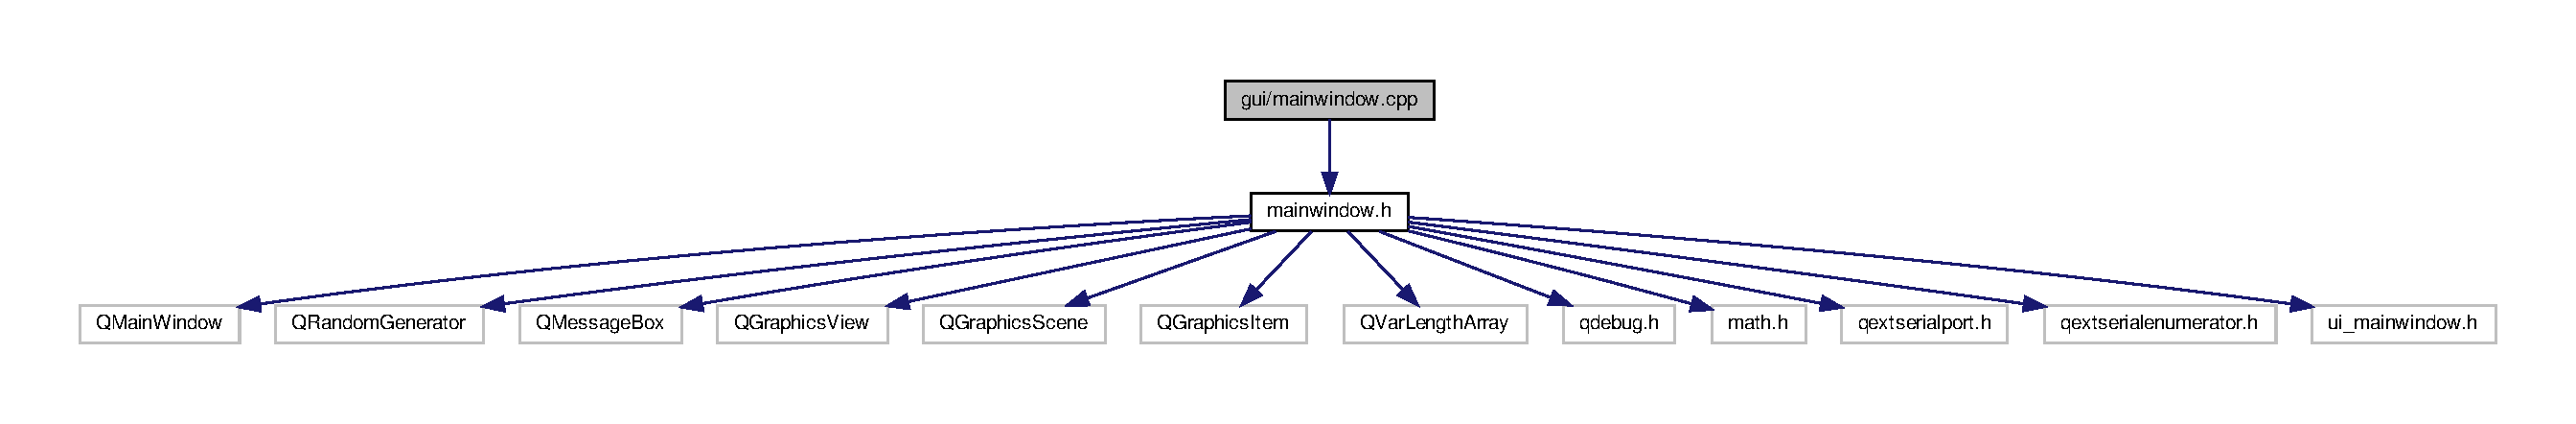
\includegraphics[width=350pt]{mainwindow_8cpp__incl}
\end{center}
\end{figure}
\subsection*{Variables}
\begin{DoxyCompactItemize}
\item 
\mbox{\Hypertarget{mainwindow_8cpp_a43016d873124d39034edb8cd164794db}\label{mainwindow_8cpp_a43016d873124d39034edb8cd164794db}} 
const double {\bfseries pi} = 3.\+14159
\item 
\mbox{\Hypertarget{mainwindow_8cpp_aacae39714d7e2bf245d994f68fb2d4fa}\label{mainwindow_8cpp_aacae39714d7e2bf245d994f68fb2d4fa}} 
const int {\bfseries n\+\_\+limit} = 100
\end{DoxyCompactItemize}


\subsection{Detailed Description}
\begin{DoxyAuthor}{Author}
Patrick Willner (\href{mailto:patrick.willner@tum.de}{\tt patrick.\+willner@tum.\+de}), Andreas Koliopoulos (\href{mailto:ga96leh@mytum.de}{\tt ga96leh@mytum.\+de}), Alexander Schmaus (\href{mailto:ga96fin@mytum.de}{\tt ga96fin@mytum.\+de}) 
\end{DoxyAuthor}
\begin{DoxyVersion}{Version}
1.\+0 
\end{DoxyVersion}
\begin{DoxyDate}{Date}
2019-\/12-\/12
\end{DoxyDate}
\begin{DoxyCopyright}{Copyright}
Copyright (c) 2019 
\end{DoxyCopyright}

\hypertarget{mainwindow_8h}{}\section{gui/mainwindow.h File Reference}
\label{mainwindow_8h}\index{gui/mainwindow.\+h@{gui/mainwindow.\+h}}
{\ttfamily \#include $<$Q\+Main\+Window$>$}\newline
{\ttfamily \#include $<$Q\+Random\+Generator$>$}\newline
{\ttfamily \#include $<$Q\+Message\+Box$>$}\newline
{\ttfamily \#include $<$Q\+Graphics\+View$>$}\newline
{\ttfamily \#include $<$Q\+Graphics\+Scene$>$}\newline
{\ttfamily \#include $<$Q\+Graphics\+Item$>$}\newline
{\ttfamily \#include $<$Q\+Var\+Length\+Array$>$}\newline
{\ttfamily \#include $<$qdebug.\+h$>$}\newline
{\ttfamily \#include $<$math.\+h$>$}\newline
{\ttfamily \#include \char`\"{}qextserialport.\+h\char`\"{}}\newline
{\ttfamily \#include \char`\"{}qextserialenumerator.\+h\char`\"{}}\newline
{\ttfamily \#include \char`\"{}ui\+\_\+mainwindow.\+h\char`\"{}}\newline
Include dependency graph for mainwindow.\+h\+:
\nopagebreak
\begin{figure}[H]
\begin{center}
\leavevmode
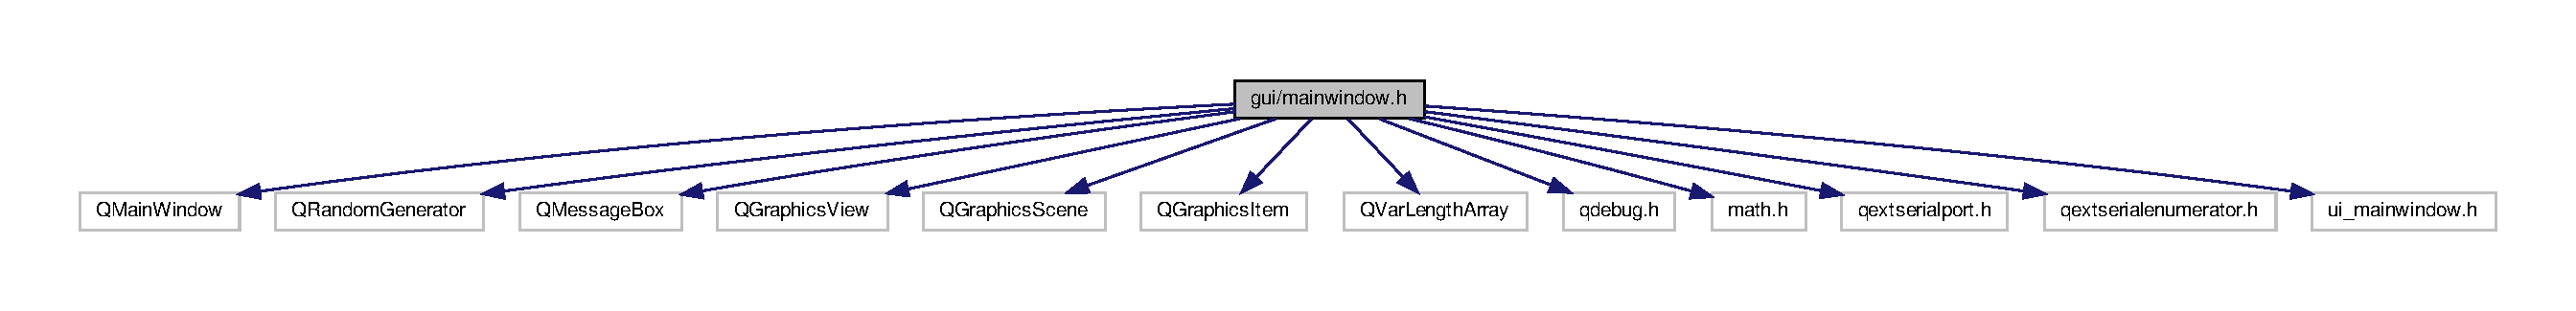
\includegraphics[width=350pt]{mainwindow_8h__incl}
\end{center}
\end{figure}
This graph shows which files directly or indirectly include this file\+:
\nopagebreak
\begin{figure}[H]
\begin{center}
\leavevmode
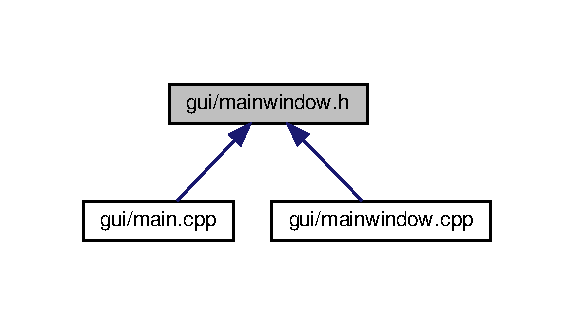
\includegraphics[width=276pt]{mainwindow_8h__dep__incl}
\end{center}
\end{figure}
\subsection*{Classes}
\begin{DoxyCompactItemize}
\item 
class \hyperlink{classMainWindow}{Main\+Window}
\begin{DoxyCompactList}\small\item\em The \hyperlink{classMainWindow}{Main\+Window} class. \end{DoxyCompactList}\end{DoxyCompactItemize}


\subsection{Detailed Description}
\begin{DoxyAuthor}{Author}
Patrick Willner (\href{mailto:patrick.willner@tum.de}{\tt patrick.\+willner@tum.\+de}), Andreas Koliopoulos (\href{mailto:ga96leh@mytum.de}{\tt ga96leh@mytum.\+de}), Alexander Schmaus (\href{mailto:ga96fin@mytum.de}{\tt ga96fin@mytum.\+de}) 
\end{DoxyAuthor}
\begin{DoxyVersion}{Version}
1.\+0 
\end{DoxyVersion}
\begin{DoxyDate}{Date}
2019-\/12-\/12
\end{DoxyDate}
\begin{DoxyCopyright}{Copyright}
Copyright (c) 2019 
\end{DoxyCopyright}

\hypertarget{mote__sensors_8c}{}\section{src/mote\+\_\+sensors.c File Reference}
\label{mote__sensors_8c}\index{src/mote\+\_\+sensors.\+c@{src/mote\+\_\+sensors.\+c}}
{\ttfamily \#include \char`\"{}mote\+\_\+sensors.\+h\char`\"{}}\newline
{\ttfamily \#include \char`\"{}routing.\+h\char`\"{}}\newline
{\ttfamily \#include $<$dev/button-\/sensor.\+h$>$}\newline
{\ttfamily \#include $<$dev/adc-\/zoul.\+h$>$}\newline
{\ttfamily \#include $<$dev/zoul-\/sensors.\+h$>$}\newline
{\ttfamily \#include $<$dev/sys-\/ctrl.\+h$>$}\newline
{\ttfamily \#include \char`\"{}cfs/cfs.\+h\char`\"{}}\newline
{\ttfamily \#include \char`\"{}clock.\+h\char`\"{}}\newline
Include dependency graph for mote\+\_\+sensors.\+c\+:\nopagebreak
\begin{figure}[H]
\begin{center}
\leavevmode
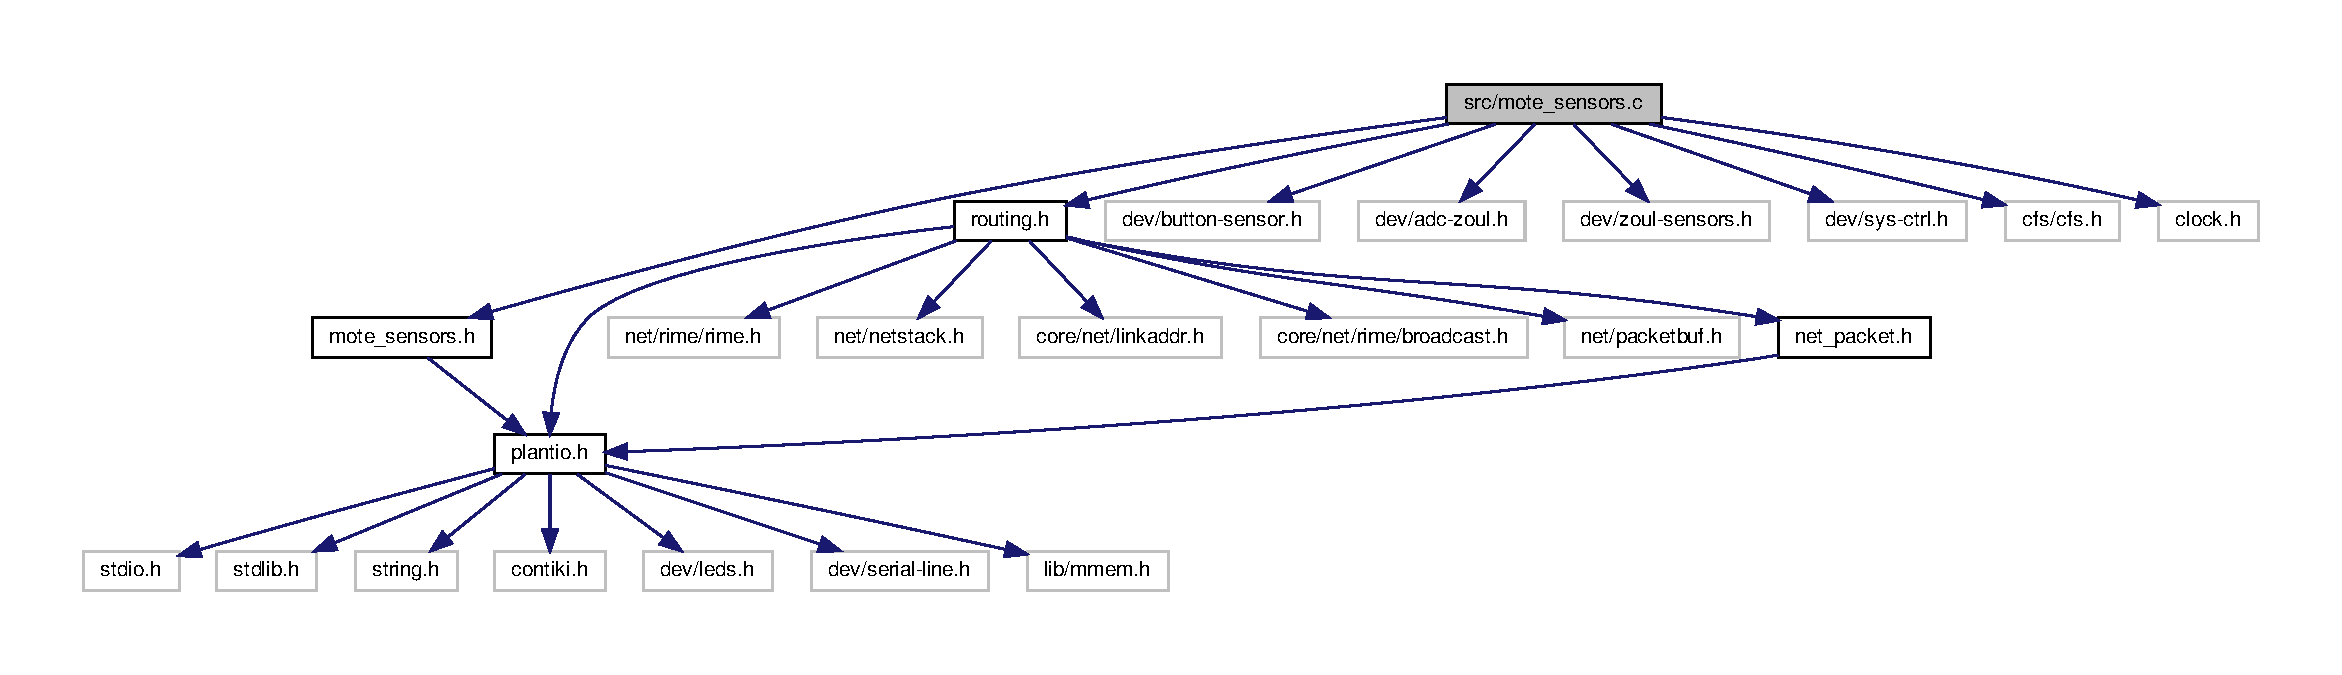
\includegraphics[width=350pt]{mote__sensors_8c__incl}
\end{center}
\end{figure}
\subsection*{Macros}
\begin{DoxyCompactItemize}
\item 
\mbox{\Hypertarget{mote__sensors_8c_ab56779ef7e65f077c58a13f09dcbbc85}\label{mote__sensors_8c_ab56779ef7e65f077c58a13f09dcbbc85}} 
\#define {\bfseries T\+E\+M\+P\+\_\+\+R\+E\+A\+D\+\_\+\+I\+N\+T\+E\+R\+V\+AL}~C\+L\+O\+C\+K\+\_\+\+S\+E\+C\+O\+ND $\ast$ 3
\end{DoxyCompactItemize}
\subsection*{Functions}
\begin{DoxyCompactItemize}
\item 
\mbox{\Hypertarget{mote__sensors_8c_a4f75e886e40e7ac5ee2ad21eadd74c0e}\label{mote__sensors_8c_a4f75e886e40e7ac5ee2ad21eadd74c0e}} 
{\bfseries P\+R\+O\+C\+E\+SS} (\hyperlink{mote__sensors_8h_acd4c513676b015a76fa25f02fed26588}{p\+\_\+sensors}, \char`\"{}\char`\"{})
\item 
\mbox{\Hypertarget{mote__sensors_8c_a2d5a918f81126d15fd3b37bf264a74dc}\label{mote__sensors_8c_a2d5a918f81126d15fd3b37bf264a74dc}} 
{\bfseries P\+R\+O\+C\+E\+S\+S\+\_\+\+T\+H\+R\+E\+AD} (\hyperlink{mote__sensors_8h_acd4c513676b015a76fa25f02fed26588}{p\+\_\+sensors}, ev, data)
\item 
\mbox{\Hypertarget{mote__sensors_8c_a68cf112f6a9b76c2ac2ff21665d5482f}\label{mote__sensors_8c_a68cf112f6a9b76c2ac2ff21665d5482f}} 
void \hyperlink{mote__sensors_8c_a68cf112f6a9b76c2ac2ff21665d5482f}{init\+\_\+sensor\+\_\+data} (void)
\begin{DoxyCompactList}\small\item\em Initializes the Device sensors thresholds. \end{DoxyCompactList}\item 
void \hyperlink{mote__sensors_8c_a261f3bfff99934d39784c9a0bd5ab1ff}{write\+\_\+sensor\+\_\+data} (const uint16\+\_\+t temp, const uint16\+\_\+t hum, const uint16\+\_\+t light)
\begin{DoxyCompactList}\small\item\em Writes a tuple of sensor data to flash memory. \end{DoxyCompactList}\item 
const uint16\+\_\+t \hyperlink{mote__sensors_8c_a8a4d789068eb286ad36928227cf54904}{fetch\+\_\+sensor\+\_\+data} (const uint16\+\_\+t index)
\begin{DoxyCompactList}\small\item\em Retrieve Sensor data from the flash memory. \end{DoxyCompactList}\item 
\mbox{\Hypertarget{mote__sensors_8c_ab74d95815434dc77b0763cfe9baa33bd}\label{mote__sensors_8c_ab74d95815434dc77b0763cfe9baa33bd}} 
void \hyperlink{mote__sensors_8c_ab74d95815434dc77b0763cfe9baa33bd}{on\+\_\+button\+\_\+pressed} (void)
\begin{DoxyCompactList}\small\item\em Handle a button press event on the device. \end{DoxyCompactList}\item 
\mbox{\Hypertarget{mote__sensors_8c_afa19d23bfc6215812436195d62ba8b99}\label{mote__sensors_8c_afa19d23bfc6215812436195d62ba8b99}} 
void \hyperlink{mote__sensors_8c_afa19d23bfc6215812436195d62ba8b99}{clear\+\_\+sensor\+\_\+data} (void)
\begin{DoxyCompactList}\small\item\em Clears all sensor data from the flash memory. \end{DoxyCompactList}\item 
\mbox{\Hypertarget{mote__sensors_8c_a4bc9bfc0677667a966d7ab73efafa4d1}\label{mote__sensors_8c_a4bc9bfc0677667a966d7ab73efafa4d1}} 
void \hyperlink{mote__sensors_8c_a4bc9bfc0677667a966d7ab73efafa4d1}{print\+\_\+sensor\+\_\+data} (void)
\begin{DoxyCompactList}\small\item\em Prints the senors data. \end{DoxyCompactList}\item 
void \hyperlink{mote__sensors_8c_a055459c78ce7052f76e74a1a0505c47b}{write\+\_\+thresholds} (char $\ast$str)
\begin{DoxyCompactList}\small\item\em Write the sensors thresholds to the flash memory. \end{DoxyCompactList}\item 
const int32\+\_\+t \hyperlink{mote__sensors_8c_a9fcd98e47b3747e0862357f869049128}{get\+\_\+threshold} (enum \hyperlink{plantio_8h_aedfc9d8254f442cb95c1b5784835ef9b}{thresh} id)
\begin{DoxyCompactList}\small\item\em Get sensor threshold value. \end{DoxyCompactList}\item 
const uint16\+\_\+t \hyperlink{mote__sensors_8c_a08a3f61c155e6217f2efb50c86a3cc3d}{get\+\_\+light\+\_\+sensor\+\_\+value} (uint16\+\_\+t adc\+\_\+input)
\begin{DoxyCompactList}\small\item\em Calculates the light sensor value in Lm. \end{DoxyCompactList}\end{DoxyCompactItemize}


\subsection{Detailed Description}
\begin{DoxyAuthor}{Author}
Patrick Willner (\href{mailto:patrick.willner@tum.de}{\tt patrick.\+willner@tum.\+de}), Andreas Koliopoulos (\href{mailto:ga96leh@mytum.de}{\tt ga96leh@mytum.\+de}), Alexander Schmaus (\href{mailto:ga96fin@mytum.de}{\tt ga96fin@mytum.\+de}) 
\end{DoxyAuthor}
\begin{DoxyVersion}{Version}
0.\+1 
\end{DoxyVersion}
\begin{DoxyDate}{Date}
2019-\/12-\/12
\end{DoxyDate}
\begin{DoxyCopyright}{Copyright}
Copyright (c) 2019 
\end{DoxyCopyright}


\subsection{Function Documentation}
\mbox{\Hypertarget{mote__sensors_8c_a8a4d789068eb286ad36928227cf54904}\label{mote__sensors_8c_a8a4d789068eb286ad36928227cf54904}} 
\index{mote\+\_\+sensors.\+c@{mote\+\_\+sensors.\+c}!fetch\+\_\+sensor\+\_\+data@{fetch\+\_\+sensor\+\_\+data}}
\index{fetch\+\_\+sensor\+\_\+data@{fetch\+\_\+sensor\+\_\+data}!mote\+\_\+sensors.\+c@{mote\+\_\+sensors.\+c}}
\subsubsection{\texorpdfstring{fetch\+\_\+sensor\+\_\+data()}{fetch\_sensor\_data()}}
{\footnotesize\ttfamily const uint16\+\_\+t fetch\+\_\+sensor\+\_\+data (\begin{DoxyParamCaption}\item[{const uint16\+\_\+t}]{index }\end{DoxyParamCaption})}



Retrieve Sensor data from the flash memory. 

First 6$\ast$4 bytes are thresholds. Next 4$\ast$2 bytes are timestamp, temp, hum, light for maximum number of M\+A\+X\+\_\+\+N\+U\+M\+\_\+\+V\+A\+L\+U\+ES


\begin{DoxyParams}{Parameters}
{\em index} & Index starting from 6$\ast$4 + Index \\
\hline
\end{DoxyParams}
\begin{DoxyReturn}{Returns}
const uint16\+\_\+t Sensors data value 
\end{DoxyReturn}
\mbox{\Hypertarget{mote__sensors_8c_a08a3f61c155e6217f2efb50c86a3cc3d}\label{mote__sensors_8c_a08a3f61c155e6217f2efb50c86a3cc3d}} 
\index{mote\+\_\+sensors.\+c@{mote\+\_\+sensors.\+c}!get\+\_\+light\+\_\+sensor\+\_\+value@{get\+\_\+light\+\_\+sensor\+\_\+value}}
\index{get\+\_\+light\+\_\+sensor\+\_\+value@{get\+\_\+light\+\_\+sensor\+\_\+value}!mote\+\_\+sensors.\+c@{mote\+\_\+sensors.\+c}}
\subsubsection{\texorpdfstring{get\+\_\+light\+\_\+sensor\+\_\+value()}{get\_light\_sensor\_value()}}
{\footnotesize\ttfamily const uint16\+\_\+t get\+\_\+light\+\_\+sensor\+\_\+value (\begin{DoxyParamCaption}\item[{uint16\+\_\+t}]{adc\+\_\+input }\end{DoxyParamCaption})}



Calculates the light sensor value in Lm. 


\begin{DoxyParams}{Parameters}
{\em adc\+\_\+input} & Voltage \\
\hline
\end{DoxyParams}
\begin{DoxyReturn}{Returns}
const uint16\+\_\+t 
\end{DoxyReturn}
\mbox{\Hypertarget{mote__sensors_8c_a9fcd98e47b3747e0862357f869049128}\label{mote__sensors_8c_a9fcd98e47b3747e0862357f869049128}} 
\index{mote\+\_\+sensors.\+c@{mote\+\_\+sensors.\+c}!get\+\_\+threshold@{get\+\_\+threshold}}
\index{get\+\_\+threshold@{get\+\_\+threshold}!mote\+\_\+sensors.\+c@{mote\+\_\+sensors.\+c}}
\subsubsection{\texorpdfstring{get\+\_\+threshold()}{get\_threshold()}}
{\footnotesize\ttfamily const int32\+\_\+t get\+\_\+threshold (\begin{DoxyParamCaption}\item[{enum \hyperlink{plantio_8h_aedfc9d8254f442cb95c1b5784835ef9b}{thresh}}]{id }\end{DoxyParamCaption})}



Get sensor threshold value. 


\begin{DoxyParams}{Parameters}
{\em id} & ID to specify which threshold, defined with enum thresh \\
\hline
\end{DoxyParams}
\begin{DoxyReturn}{Returns}
const int32\+\_\+t sensors threshold value 
\end{DoxyReturn}
\mbox{\Hypertarget{mote__sensors_8c_a261f3bfff99934d39784c9a0bd5ab1ff}\label{mote__sensors_8c_a261f3bfff99934d39784c9a0bd5ab1ff}} 
\index{mote\+\_\+sensors.\+c@{mote\+\_\+sensors.\+c}!write\+\_\+sensor\+\_\+data@{write\+\_\+sensor\+\_\+data}}
\index{write\+\_\+sensor\+\_\+data@{write\+\_\+sensor\+\_\+data}!mote\+\_\+sensors.\+c@{mote\+\_\+sensors.\+c}}
\subsubsection{\texorpdfstring{write\+\_\+sensor\+\_\+data()}{write\_sensor\_data()}}
{\footnotesize\ttfamily void write\+\_\+sensor\+\_\+data (\begin{DoxyParamCaption}\item[{const uint16\+\_\+t}]{temp,  }\item[{const uint16\+\_\+t}]{hum,  }\item[{const uint16\+\_\+t}]{light }\end{DoxyParamCaption})}



Writes a tuple of sensor data to flash memory. 

Appends the data to the file on flash memory and assigns the tuple a unique timestamp. Only keeps the latest M\+A\+X\+\_\+\+N\+U\+M\+\_\+\+O\+F\+\_\+\+V\+A\+L\+U\+ES number of values.


\begin{DoxyParams}{Parameters}
{\em temp} & Temperatur value \\
\hline
{\em hum} & Humidity value \\
\hline
{\em light} & Light value \\
\hline
\end{DoxyParams}
\mbox{\Hypertarget{mote__sensors_8c_a055459c78ce7052f76e74a1a0505c47b}\label{mote__sensors_8c_a055459c78ce7052f76e74a1a0505c47b}} 
\index{mote\+\_\+sensors.\+c@{mote\+\_\+sensors.\+c}!write\+\_\+thresholds@{write\+\_\+thresholds}}
\index{write\+\_\+thresholds@{write\+\_\+thresholds}!mote\+\_\+sensors.\+c@{mote\+\_\+sensors.\+c}}
\subsubsection{\texorpdfstring{write\+\_\+thresholds()}{write\_thresholds()}}
{\footnotesize\ttfamily void write\+\_\+thresholds (\begin{DoxyParamCaption}\item[{char $\ast$}]{str }\end{DoxyParamCaption})}



Write the sensors thresholds to the flash memory. 


\begin{DoxyParams}{Parameters}
{\em str} & Threshold as string formatted, seperated by \textquotesingle{}\+:\textquotesingle{} \\
\hline
\end{DoxyParams}

\hypertarget{mote__sensors_8h}{}\section{src/mote\+\_\+sensors.h File Reference}
\label{mote__sensors_8h}\index{src/mote\+\_\+sensors.\+h@{src/mote\+\_\+sensors.\+h}}
{\ttfamily \#include \char`\"{}plantio.\+h\char`\"{}}\newline
Include dependency graph for mote\+\_\+sensors.\+h\+:
\nopagebreak
\begin{figure}[H]
\begin{center}
\leavevmode
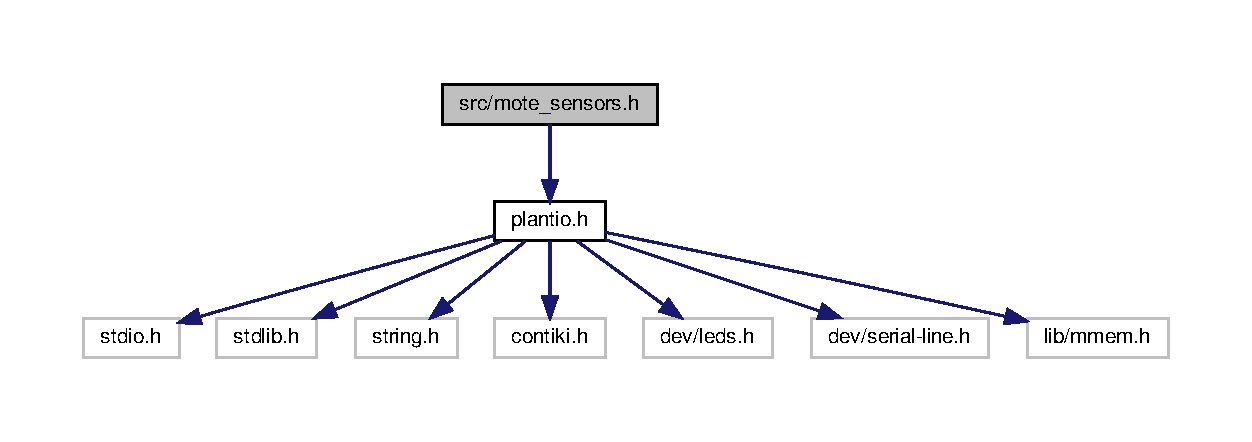
\includegraphics[width=350pt]{mote__sensors_8h__incl}
\end{center}
\end{figure}
This graph shows which files directly or indirectly include this file\+:
\nopagebreak
\begin{figure}[H]
\begin{center}
\leavevmode
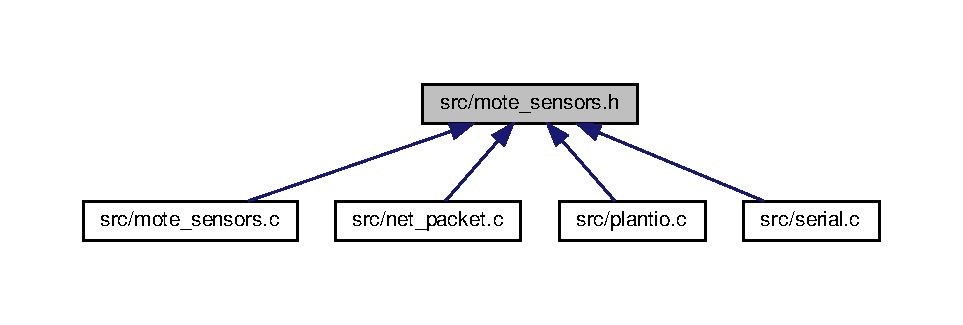
\includegraphics[width=350pt]{mote__sensors_8h__dep__incl}
\end{center}
\end{figure}
\subsection*{Functions}
\begin{DoxyCompactItemize}
\item 
\mbox{\Hypertarget{mote__sensors_8h_ab74d95815434dc77b0763cfe9baa33bd}\label{mote__sensors_8h_ab74d95815434dc77b0763cfe9baa33bd}} 
void \hyperlink{mote__sensors_8h_ab74d95815434dc77b0763cfe9baa33bd}{on\+\_\+button\+\_\+pressed} (void)
\begin{DoxyCompactList}\small\item\em Handle a button press event on the device. \end{DoxyCompactList}\item 
const uint16\+\_\+t \hyperlink{mote__sensors_8h_a08a3f61c155e6217f2efb50c86a3cc3d}{get\+\_\+light\+\_\+sensor\+\_\+value} (uint16\+\_\+t adc\+\_\+input)
\begin{DoxyCompactList}\small\item\em Calculates the light sensor value in Lm. \end{DoxyCompactList}\item 
\mbox{\Hypertarget{mote__sensors_8h_a68cf112f6a9b76c2ac2ff21665d5482f}\label{mote__sensors_8h_a68cf112f6a9b76c2ac2ff21665d5482f}} 
void \hyperlink{mote__sensors_8h_a68cf112f6a9b76c2ac2ff21665d5482f}{init\+\_\+sensor\+\_\+data} (void)
\begin{DoxyCompactList}\small\item\em Initializes the Device sensors thresholds. \end{DoxyCompactList}\item 
void \hyperlink{mote__sensors_8h_a261f3bfff99934d39784c9a0bd5ab1ff}{write\+\_\+sensor\+\_\+data} (const uint16\+\_\+t temp, const uint16\+\_\+t hum, const uint16\+\_\+t light)
\begin{DoxyCompactList}\small\item\em Writes a tuple of sensor data to flash memory. \end{DoxyCompactList}\item 
\mbox{\Hypertarget{mote__sensors_8h_afa19d23bfc6215812436195d62ba8b99}\label{mote__sensors_8h_afa19d23bfc6215812436195d62ba8b99}} 
void \hyperlink{mote__sensors_8h_afa19d23bfc6215812436195d62ba8b99}{clear\+\_\+sensor\+\_\+data} (void)
\begin{DoxyCompactList}\small\item\em Clears all sensor data from the flash memory. \end{DoxyCompactList}\item 
\mbox{\Hypertarget{mote__sensors_8h_a4bc9bfc0677667a966d7ab73efafa4d1}\label{mote__sensors_8h_a4bc9bfc0677667a966d7ab73efafa4d1}} 
void \hyperlink{mote__sensors_8h_a4bc9bfc0677667a966d7ab73efafa4d1}{print\+\_\+sensor\+\_\+data} (void)
\begin{DoxyCompactList}\small\item\em Prints the senors data. \end{DoxyCompactList}\item 
const uint16\+\_\+t \hyperlink{mote__sensors_8h_a8a4d789068eb286ad36928227cf54904}{fetch\+\_\+sensor\+\_\+data} (const uint16\+\_\+t index)
\begin{DoxyCompactList}\small\item\em Retrieve Sensor data from the flash memory. \end{DoxyCompactList}\item 
void \hyperlink{mote__sensors_8h_a055459c78ce7052f76e74a1a0505c47b}{write\+\_\+thresholds} (char $\ast$str)
\begin{DoxyCompactList}\small\item\em Write the sensors thresholds to the flash memory. \end{DoxyCompactList}\item 
const int32\+\_\+t \hyperlink{mote__sensors_8h_a9fcd98e47b3747e0862357f869049128}{get\+\_\+threshold} (enum \hyperlink{plantio_8h_aedfc9d8254f442cb95c1b5784835ef9b}{thresh} id)
\begin{DoxyCompactList}\small\item\em Get sensor threshold value. \end{DoxyCompactList}\end{DoxyCompactItemize}
\subsection*{Variables}
\begin{DoxyCompactItemize}
\item 
\mbox{\Hypertarget{mote__sensors_8h_acd4c513676b015a76fa25f02fed26588}\label{mote__sensors_8h_acd4c513676b015a76fa25f02fed26588}} 
struct process \hyperlink{mote__sensors_8h_acd4c513676b015a76fa25f02fed26588}{p\+\_\+sensors}
\begin{DoxyCompactList}\small\item\em Process for periodically saving sensors data. \end{DoxyCompactList}\end{DoxyCompactItemize}


\subsection{Detailed Description}
\begin{DoxyAuthor}{Author}
Patrick Willner (\href{mailto:patrick.willner@tum.de}{\tt patrick.\+willner@tum.\+de}), Andreas Koliopoulos (\href{mailto:ga96leh@mytum.de}{\tt ga96leh@mytum.\+de}), Alexander Schmaus (\href{mailto:ga96fin@mytum.de}{\tt ga96fin@mytum.\+de}) 
\end{DoxyAuthor}
\begin{DoxyVersion}{Version}
0.\+1 
\end{DoxyVersion}
\begin{DoxyDate}{Date}
2019-\/12-\/12
\end{DoxyDate}
\begin{DoxyCopyright}{Copyright}
Copyright (c) 2019 
\end{DoxyCopyright}


\subsection{Function Documentation}
\mbox{\Hypertarget{mote__sensors_8h_a8a4d789068eb286ad36928227cf54904}\label{mote__sensors_8h_a8a4d789068eb286ad36928227cf54904}} 
\index{mote\+\_\+sensors.\+h@{mote\+\_\+sensors.\+h}!fetch\+\_\+sensor\+\_\+data@{fetch\+\_\+sensor\+\_\+data}}
\index{fetch\+\_\+sensor\+\_\+data@{fetch\+\_\+sensor\+\_\+data}!mote\+\_\+sensors.\+h@{mote\+\_\+sensors.\+h}}
\subsubsection{\texorpdfstring{fetch\+\_\+sensor\+\_\+data()}{fetch\_sensor\_data()}}
{\footnotesize\ttfamily const uint16\+\_\+t fetch\+\_\+sensor\+\_\+data (\begin{DoxyParamCaption}\item[{const uint16\+\_\+t}]{index }\end{DoxyParamCaption})}



Retrieve Sensor data from the flash memory. 

First 6$\ast$4 bytes are thresholds. Next 4$\ast$2 bytes are timestamp, temp, hum, light for maximum number of M\+A\+X\+\_\+\+N\+U\+M\+\_\+\+V\+A\+L\+U\+ES


\begin{DoxyParams}{Parameters}
{\em index} & Index starting from 6$\ast$4 + Index \\
\hline
\end{DoxyParams}
\begin{DoxyReturn}{Returns}
const uint16\+\_\+t Sensors data value 
\end{DoxyReturn}
\mbox{\Hypertarget{mote__sensors_8h_a08a3f61c155e6217f2efb50c86a3cc3d}\label{mote__sensors_8h_a08a3f61c155e6217f2efb50c86a3cc3d}} 
\index{mote\+\_\+sensors.\+h@{mote\+\_\+sensors.\+h}!get\+\_\+light\+\_\+sensor\+\_\+value@{get\+\_\+light\+\_\+sensor\+\_\+value}}
\index{get\+\_\+light\+\_\+sensor\+\_\+value@{get\+\_\+light\+\_\+sensor\+\_\+value}!mote\+\_\+sensors.\+h@{mote\+\_\+sensors.\+h}}
\subsubsection{\texorpdfstring{get\+\_\+light\+\_\+sensor\+\_\+value()}{get\_light\_sensor\_value()}}
{\footnotesize\ttfamily const uint16\+\_\+t get\+\_\+light\+\_\+sensor\+\_\+value (\begin{DoxyParamCaption}\item[{uint16\+\_\+t}]{adc\+\_\+input }\end{DoxyParamCaption})}



Calculates the light sensor value in Lm. 


\begin{DoxyParams}{Parameters}
{\em adc\+\_\+input} & Voltage \\
\hline
\end{DoxyParams}
\begin{DoxyReturn}{Returns}
const uint16\+\_\+t 
\end{DoxyReturn}
\mbox{\Hypertarget{mote__sensors_8h_a9fcd98e47b3747e0862357f869049128}\label{mote__sensors_8h_a9fcd98e47b3747e0862357f869049128}} 
\index{mote\+\_\+sensors.\+h@{mote\+\_\+sensors.\+h}!get\+\_\+threshold@{get\+\_\+threshold}}
\index{get\+\_\+threshold@{get\+\_\+threshold}!mote\+\_\+sensors.\+h@{mote\+\_\+sensors.\+h}}
\subsubsection{\texorpdfstring{get\+\_\+threshold()}{get\_threshold()}}
{\footnotesize\ttfamily const int32\+\_\+t get\+\_\+threshold (\begin{DoxyParamCaption}\item[{enum \hyperlink{plantio_8h_aedfc9d8254f442cb95c1b5784835ef9b}{thresh}}]{id }\end{DoxyParamCaption})}



Get sensor threshold value. 


\begin{DoxyParams}{Parameters}
{\em id} & ID to specify which threshold, defined with enum thresh \\
\hline
\end{DoxyParams}
\begin{DoxyReturn}{Returns}
const int32\+\_\+t sensors threshold value 
\end{DoxyReturn}
\mbox{\Hypertarget{mote__sensors_8h_a261f3bfff99934d39784c9a0bd5ab1ff}\label{mote__sensors_8h_a261f3bfff99934d39784c9a0bd5ab1ff}} 
\index{mote\+\_\+sensors.\+h@{mote\+\_\+sensors.\+h}!write\+\_\+sensor\+\_\+data@{write\+\_\+sensor\+\_\+data}}
\index{write\+\_\+sensor\+\_\+data@{write\+\_\+sensor\+\_\+data}!mote\+\_\+sensors.\+h@{mote\+\_\+sensors.\+h}}
\subsubsection{\texorpdfstring{write\+\_\+sensor\+\_\+data()}{write\_sensor\_data()}}
{\footnotesize\ttfamily void write\+\_\+sensor\+\_\+data (\begin{DoxyParamCaption}\item[{const uint16\+\_\+t}]{temp,  }\item[{const uint16\+\_\+t}]{hum,  }\item[{const uint16\+\_\+t}]{light }\end{DoxyParamCaption})}



Writes a tuple of sensor data to flash memory. 

Appends the data to the file on flash memory and assigns the tuple a unique timestamp. Only keeps the latest M\+A\+X\+\_\+\+N\+U\+M\+\_\+\+O\+F\+\_\+\+V\+A\+L\+U\+ES number of values.


\begin{DoxyParams}{Parameters}
{\em temp} & Temperatur value \\
\hline
{\em hum} & Humidity value \\
\hline
{\em light} & Light value \\
\hline
\end{DoxyParams}
\mbox{\Hypertarget{mote__sensors_8h_a055459c78ce7052f76e74a1a0505c47b}\label{mote__sensors_8h_a055459c78ce7052f76e74a1a0505c47b}} 
\index{mote\+\_\+sensors.\+h@{mote\+\_\+sensors.\+h}!write\+\_\+thresholds@{write\+\_\+thresholds}}
\index{write\+\_\+thresholds@{write\+\_\+thresholds}!mote\+\_\+sensors.\+h@{mote\+\_\+sensors.\+h}}
\subsubsection{\texorpdfstring{write\+\_\+thresholds()}{write\_thresholds()}}
{\footnotesize\ttfamily void write\+\_\+thresholds (\begin{DoxyParamCaption}\item[{char $\ast$}]{str }\end{DoxyParamCaption})}



Write the sensors thresholds to the flash memory. 


\begin{DoxyParams}{Parameters}
{\em str} & Threshold as string formatted, seperated by \textquotesingle{}\+:\textquotesingle{} \\
\hline
\end{DoxyParams}

\hypertarget{net__packet_8c}{}\section{src/net\+\_\+packet.c File Reference}
\label{net__packet_8c}\index{src/net\+\_\+packet.\+c@{src/net\+\_\+packet.\+c}}
{\ttfamily \#include \char`\"{}net\+\_\+packet.\+h\char`\"{}}\newline
{\ttfamily \#include \char`\"{}routing.\+h\char`\"{}}\newline
{\ttfamily \#include \char`\"{}mote\+\_\+sensors.\+h\char`\"{}}\newline
{\ttfamily \#include \char`\"{}cfs/cfs.\+h\char`\"{}}\newline
Include dependency graph for net\+\_\+packet.\+c\+:\nopagebreak
\begin{figure}[H]
\begin{center}
\leavevmode
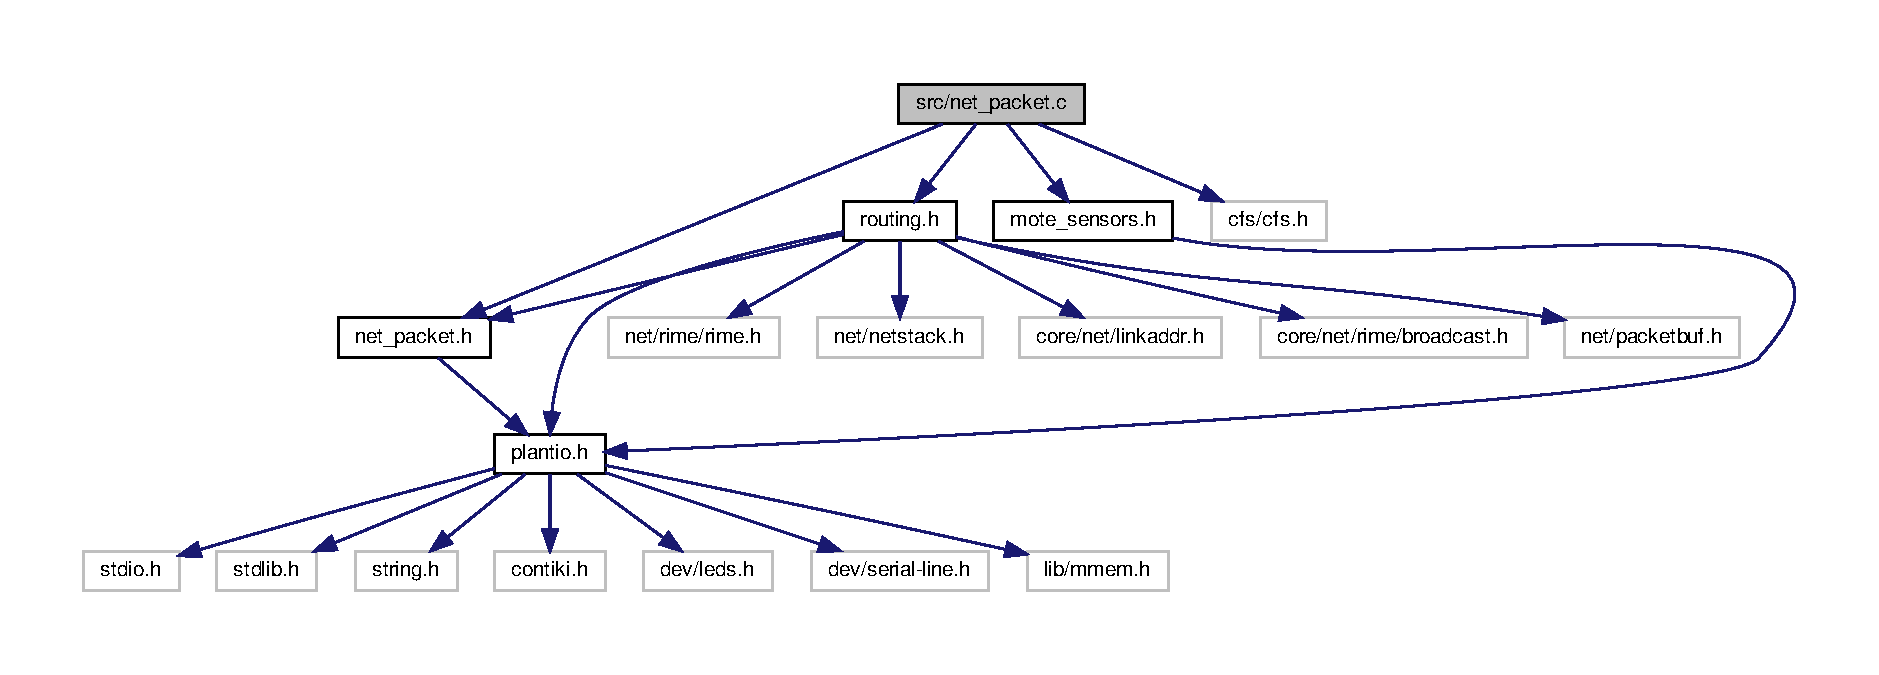
\includegraphics[width=350pt]{net__packet_8c__incl}
\end{center}
\end{figure}
\subsection*{Functions}
\begin{DoxyCompactItemize}
\item 
int \hyperlink{net__packet_8c_a5fd67a775b8716b6b7b72b61674b5bbd}{create\+\_\+packet} (const uint8\+\_\+t type, const uint8\+\_\+t $\ast$src, uint8\+\_\+t src\+\_\+len, const uint8\+\_\+t $\ast$dest, uint8\+\_\+t dest\+\_\+len, const uint8\+\_\+t $\ast$data, uint8\+\_\+t data\+\_\+len)
\begin{DoxyCompactList}\small\item\em Create a packet object and dynamically allocates memory given by the size of the data. \end{DoxyCompactList}\item 
void \hyperlink{net__packet_8c_a18a89d38116621e0446c8873ee8dc2bb}{print\+\_\+packet} (const plantio\+\_\+packet\+\_\+t $\ast$packet)
\begin{DoxyCompactList}\small\item\em Prints packet information. \end{DoxyCompactList}\item 
\mbox{\Hypertarget{net__packet_8c_a45c6c1870fed33abf147e85fb1537981}\label{net__packet_8c_a45c6c1870fed33abf147e85fb1537981}} 
const uint8\+\_\+t $\ast$ {\bfseries get\+\_\+packet\+\_\+src} (const plantio\+\_\+packet\+\_\+t $\ast$packet)
\item 
\mbox{\Hypertarget{net__packet_8c_a4bac7cbdf4f3042d87b7c883d64c8afd}\label{net__packet_8c_a4bac7cbdf4f3042d87b7c883d64c8afd}} 
const uint8\+\_\+t $\ast$ {\bfseries get\+\_\+packet\+\_\+dest} (const plantio\+\_\+packet\+\_\+t $\ast$packet)
\item 
\mbox{\Hypertarget{net__packet_8c_a8b2fa6d28227cfb32996c3c974e2bf2d}\label{net__packet_8c_a8b2fa6d28227cfb32996c3c974e2bf2d}} 
const uint8\+\_\+t $\ast$ {\bfseries get\+\_\+packet\+\_\+data} (const plantio\+\_\+packet\+\_\+t $\ast$packet)
\item 
void \hyperlink{net__packet_8c_ab587b8f8707a216cd988f658f688cb20}{process\+\_\+data\+\_\+packet} (const plantio\+\_\+packet\+\_\+t $\ast$packet)
\begin{DoxyCompactList}\small\item\em Processes packets with id $>$= 10. \end{DoxyCompactList}\end{DoxyCompactItemize}


\subsection{Detailed Description}
\begin{DoxyAuthor}{Author}
Patrick Willner (\href{mailto:patrick.willner@tum.de}{\tt patrick.\+willner@tum.\+de}), Andreas Koliopoulos (\href{mailto:ga96leh@mytum.de}{\tt ga96leh@mytum.\+de}), Alexander Schmaus (\href{mailto:ga96fin@mytum.de}{\tt ga96fin@mytum.\+de}) 
\end{DoxyAuthor}
\begin{DoxyVersion}{Version}
0.\+1 
\end{DoxyVersion}
\begin{DoxyDate}{Date}
2019-\/12-\/12
\end{DoxyDate}
\begin{DoxyCopyright}{Copyright}
Copyright (c) 2019 
\end{DoxyCopyright}


\subsection{Function Documentation}
\mbox{\Hypertarget{net__packet_8c_a5fd67a775b8716b6b7b72b61674b5bbd}\label{net__packet_8c_a5fd67a775b8716b6b7b72b61674b5bbd}} 
\index{net\+\_\+packet.\+c@{net\+\_\+packet.\+c}!create\+\_\+packet@{create\+\_\+packet}}
\index{create\+\_\+packet@{create\+\_\+packet}!net\+\_\+packet.\+c@{net\+\_\+packet.\+c}}
\subsubsection{\texorpdfstring{create\+\_\+packet()}{create\_packet()}}
{\footnotesize\ttfamily int create\+\_\+packet (\begin{DoxyParamCaption}\item[{const uint8\+\_\+t}]{type,  }\item[{const uint8\+\_\+t $\ast$}]{src,  }\item[{uint8\+\_\+t}]{src\+\_\+len,  }\item[{const uint8\+\_\+t $\ast$}]{dest,  }\item[{uint8\+\_\+t}]{dest\+\_\+len,  }\item[{const uint8\+\_\+t $\ast$}]{data,  }\item[{uint8\+\_\+t}]{data\+\_\+len }\end{DoxyParamCaption})}



Create a packet object and dynamically allocates memory given by the size of the data. 

The following packet types are defined\+: 0 ==$>$ \mbox{[}Broadcast\mbox{]} Network discovery packet

1 ==$>$ \mbox{[}Unicast\mbox{]} Route Request (R\+R\+EQ) Reply packet

2 ==$>$ \mbox{[}Broadcast\mbox{]} Request for the best route of the neighbouring nodes

3 ==$>$ \mbox{[}Unicast\mbox{]} Reply with the best route to new integrated node

4 ==$>$ \mbox{[}Unicast\mbox{]} A\+CK packet

$>$=10 ==$>$ \mbox{[}Unicast\mbox{]} General Data


\begin{DoxyParams}{Parameters}
{\em type} & Type of packet \\
\hline
{\em src} & Array of source addresses, i.\+e. node ids \\
\hline
{\em src\+\_\+len} & Length of array \\
\hline
{\em dest} & Array of destination addresses, i.\+e. node ids \\
\hline
{\em dest\+\_\+len} & Length of array \\
\hline
{\em data} & Array of payload as char array \\
\hline
{\em data\+\_\+len} & Length of data \\
\hline
\end{DoxyParams}
\begin{DoxyReturn}{Returns}
int Number of Bytes copied into the buffer 
\end{DoxyReturn}
\mbox{\Hypertarget{net__packet_8c_a18a89d38116621e0446c8873ee8dc2bb}\label{net__packet_8c_a18a89d38116621e0446c8873ee8dc2bb}} 
\index{net\+\_\+packet.\+c@{net\+\_\+packet.\+c}!print\+\_\+packet@{print\+\_\+packet}}
\index{print\+\_\+packet@{print\+\_\+packet}!net\+\_\+packet.\+c@{net\+\_\+packet.\+c}}
\subsubsection{\texorpdfstring{print\+\_\+packet()}{print\_packet()}}
{\footnotesize\ttfamily void print\+\_\+packet (\begin{DoxyParamCaption}\item[{const plantio\+\_\+packet\+\_\+t $\ast$}]{packet }\end{DoxyParamCaption})}



Prints packet information. 


\begin{DoxyParams}{Parameters}
{\em packet} & Instance of packet struct \\
\hline
\end{DoxyParams}
\mbox{\Hypertarget{net__packet_8c_ab587b8f8707a216cd988f658f688cb20}\label{net__packet_8c_ab587b8f8707a216cd988f658f688cb20}} 
\index{net\+\_\+packet.\+c@{net\+\_\+packet.\+c}!process\+\_\+data\+\_\+packet@{process\+\_\+data\+\_\+packet}}
\index{process\+\_\+data\+\_\+packet@{process\+\_\+data\+\_\+packet}!net\+\_\+packet.\+c@{net\+\_\+packet.\+c}}
\subsubsection{\texorpdfstring{process\+\_\+data\+\_\+packet()}{process\_data\_packet()}}
{\footnotesize\ttfamily void process\+\_\+data\+\_\+packet (\begin{DoxyParamCaption}\item[{const plantio\+\_\+packet\+\_\+t $\ast$}]{packet }\end{DoxyParamCaption})}



Processes packets with id $>$= 10. 


\begin{DoxyParams}{Parameters}
{\em packet} & Instance of packet struct \\
\hline
\end{DoxyParams}

\hypertarget{net__packet_8h}{}\section{src/net\+\_\+packet.h File Reference}
\label{net__packet_8h}\index{src/net\+\_\+packet.\+h@{src/net\+\_\+packet.\+h}}
{\ttfamily \#include \char`\"{}plantio.\+h\char`\"{}}\newline
Include dependency graph for net\+\_\+packet.\+h\+:\nopagebreak
\begin{figure}[H]
\begin{center}
\leavevmode
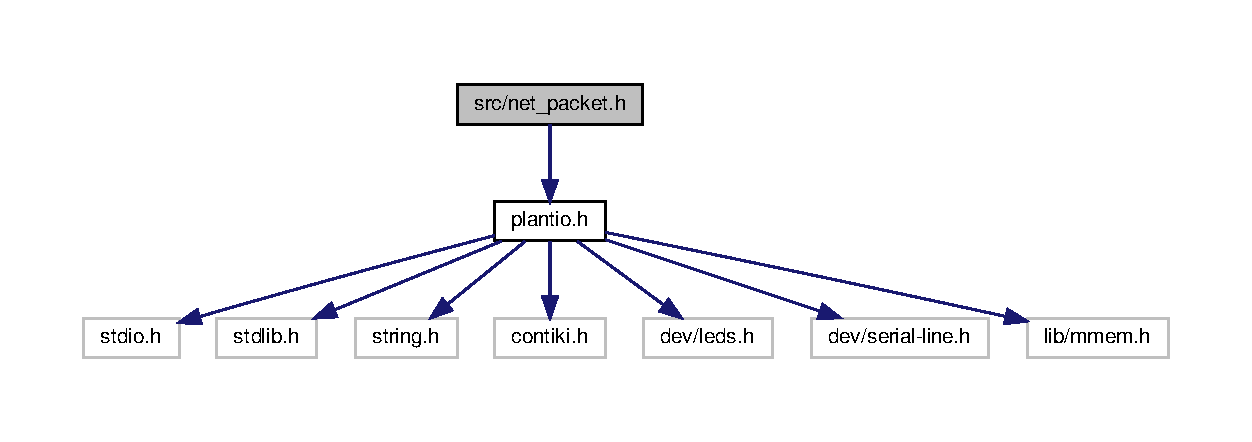
\includegraphics[width=350pt]{net__packet_8h__incl}
\end{center}
\end{figure}
This graph shows which files directly or indirectly include this file\+:\nopagebreak
\begin{figure}[H]
\begin{center}
\leavevmode
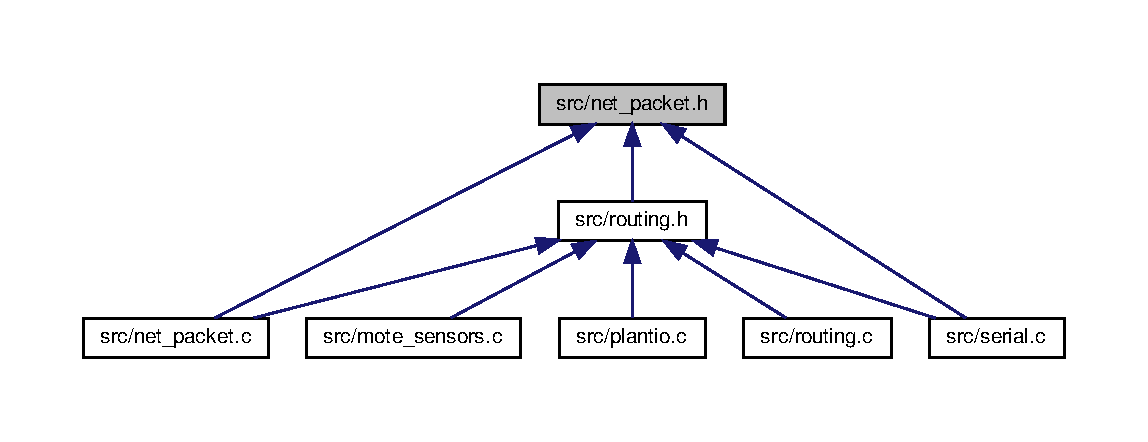
\includegraphics[width=350pt]{net__packet_8h__dep__incl}
\end{center}
\end{figure}
\subsection*{Functions}
\begin{DoxyCompactItemize}
\item 
struct \hyperlink{net__packet_8h_ad09246453a4dabd919c7541484046a87}{\+\_\+\+\_\+attribute\+\_\+\+\_\+} ((\+\_\+\+\_\+packed\+\_\+\+\_\+))
\begin{DoxyCompactList}\small\item\em General packet declaration. \end{DoxyCompactList}\item 
int \hyperlink{net__packet_8h_a5fd67a775b8716b6b7b72b61674b5bbd}{create\+\_\+packet} (const uint8\+\_\+t type, const uint8\+\_\+t $\ast$src, uint8\+\_\+t src\+\_\+len, const uint8\+\_\+t $\ast$dest, uint8\+\_\+t dest\+\_\+len, const uint8\+\_\+t $\ast$data, uint8\+\_\+t data\+\_\+len)
\begin{DoxyCompactList}\small\item\em Create a packet object and dynamically allocates memory given by the size of the data. \end{DoxyCompactList}\item 
void \hyperlink{net__packet_8h_a18a89d38116621e0446c8873ee8dc2bb}{print\+\_\+packet} (const plantio\+\_\+packet\+\_\+t $\ast$packet)
\begin{DoxyCompactList}\small\item\em Prints packet information. \end{DoxyCompactList}\item 
\mbox{\Hypertarget{net__packet_8h_a45c6c1870fed33abf147e85fb1537981}\label{net__packet_8h_a45c6c1870fed33abf147e85fb1537981}} 
const uint8\+\_\+t $\ast$ {\bfseries get\+\_\+packet\+\_\+src} (const plantio\+\_\+packet\+\_\+t $\ast$packet)
\item 
\mbox{\Hypertarget{net__packet_8h_a4bac7cbdf4f3042d87b7c883d64c8afd}\label{net__packet_8h_a4bac7cbdf4f3042d87b7c883d64c8afd}} 
const uint8\+\_\+t $\ast$ {\bfseries get\+\_\+packet\+\_\+dest} (const plantio\+\_\+packet\+\_\+t $\ast$packet)
\item 
\mbox{\Hypertarget{net__packet_8h_a8b2fa6d28227cfb32996c3c974e2bf2d}\label{net__packet_8h_a8b2fa6d28227cfb32996c3c974e2bf2d}} 
const uint8\+\_\+t $\ast$ {\bfseries get\+\_\+packet\+\_\+data} (const plantio\+\_\+packet\+\_\+t $\ast$packet)
\item 
void \hyperlink{net__packet_8h_ab587b8f8707a216cd988f658f688cb20}{process\+\_\+data\+\_\+packet} (const plantio\+\_\+packet\+\_\+t $\ast$packet)
\begin{DoxyCompactList}\small\item\em Processes packets with id $>$= 10. \end{DoxyCompactList}\end{DoxyCompactItemize}
\subsection*{Variables}
\begin{DoxyCompactItemize}
\item 
\mbox{\Hypertarget{net__packet_8h_a8677e0af94ca73f5ab833bdab56267de}\label{net__packet_8h_a8677e0af94ca73f5ab833bdab56267de}} 
typedef {\bfseries plantio\+\_\+packet\+\_\+t}
\end{DoxyCompactItemize}


\subsection{Detailed Description}
\begin{DoxyAuthor}{Author}
Patrick Willner (\href{mailto:patrick.willner@tum.de}{\tt patrick.\+willner@tum.\+de}), Andreas Koliopoulos (\href{mailto:ga96leh@mytum.de}{\tt ga96leh@mytum.\+de}), Alexander Schmaus (\href{mailto:ga96fin@mytum.de}{\tt ga96fin@mytum.\+de}) 
\end{DoxyAuthor}
\begin{DoxyVersion}{Version}
0.\+1 
\end{DoxyVersion}
\begin{DoxyDate}{Date}
2019-\/12-\/12
\end{DoxyDate}
\begin{DoxyCopyright}{Copyright}
Copyright (c) 2019 
\end{DoxyCopyright}


\subsection{Function Documentation}
\mbox{\Hypertarget{net__packet_8h_ad09246453a4dabd919c7541484046a87}\label{net__packet_8h_ad09246453a4dabd919c7541484046a87}} 
\index{net\+\_\+packet.\+h@{net\+\_\+packet.\+h}!\+\_\+\+\_\+attribute\+\_\+\+\_\+@{\+\_\+\+\_\+attribute\+\_\+\+\_\+}}
\index{\+\_\+\+\_\+attribute\+\_\+\+\_\+@{\+\_\+\+\_\+attribute\+\_\+\+\_\+}!net\+\_\+packet.\+h@{net\+\_\+packet.\+h}}
\subsubsection{\texorpdfstring{\+\_\+\+\_\+attribute\+\_\+\+\_\+()}{\_\_attribute\_\_()}}
{\footnotesize\ttfamily struct \+\_\+\+\_\+attribute\+\_\+\+\_\+ (\begin{DoxyParamCaption}\item[{(\+\_\+\+\_\+packed\+\_\+\+\_\+)}]{ }\end{DoxyParamCaption})}



General packet declaration. 

The packets are defined by a specific type, e.\+g. R\+R\+EQ packet, A\+CK, etc... The source of the packet is given by an array of Node ID. The destination, i.\+e. the path, is defined by an array. A data pointer is given to reference the payload. \mbox{\Hypertarget{net__packet_8h_a5fd67a775b8716b6b7b72b61674b5bbd}\label{net__packet_8h_a5fd67a775b8716b6b7b72b61674b5bbd}} 
\index{net\+\_\+packet.\+h@{net\+\_\+packet.\+h}!create\+\_\+packet@{create\+\_\+packet}}
\index{create\+\_\+packet@{create\+\_\+packet}!net\+\_\+packet.\+h@{net\+\_\+packet.\+h}}
\subsubsection{\texorpdfstring{create\+\_\+packet()}{create\_packet()}}
{\footnotesize\ttfamily int create\+\_\+packet (\begin{DoxyParamCaption}\item[{const uint8\+\_\+t}]{type,  }\item[{const uint8\+\_\+t $\ast$}]{src,  }\item[{uint8\+\_\+t}]{src\+\_\+len,  }\item[{const uint8\+\_\+t $\ast$}]{dest,  }\item[{uint8\+\_\+t}]{dest\+\_\+len,  }\item[{const uint8\+\_\+t $\ast$}]{data,  }\item[{uint8\+\_\+t}]{data\+\_\+len }\end{DoxyParamCaption})}



Create a packet object and dynamically allocates memory given by the size of the data. 

The following packet types are defined\+: 0 ==$>$ \mbox{[}Broadcast\mbox{]} Network discovery packet

1 ==$>$ \mbox{[}Unicast\mbox{]} Route Request (R\+R\+EQ) Reply packet

2 ==$>$ \mbox{[}Broadcast\mbox{]} Request for the best route of the neighbouring nodes

3 ==$>$ \mbox{[}Unicast\mbox{]} Reply with the best route to new integrated node

4 ==$>$ \mbox{[}Unicast\mbox{]} A\+CK packet

$>$=10 ==$>$ \mbox{[}Unicast\mbox{]} General Data


\begin{DoxyParams}{Parameters}
{\em type} & Type of packet \\
\hline
{\em src} & Array of source addresses, i.\+e. node ids \\
\hline
{\em src\+\_\+len} & Length of array \\
\hline
{\em dest} & Array of destination addresses, i.\+e. node ids \\
\hline
{\em dest\+\_\+len} & Length of array \\
\hline
{\em data} & Array of payload as char array \\
\hline
{\em data\+\_\+len} & Length of data \\
\hline
\end{DoxyParams}
\begin{DoxyReturn}{Returns}
int Number of Bytes copied into the buffer 
\end{DoxyReturn}
\mbox{\Hypertarget{net__packet_8h_a18a89d38116621e0446c8873ee8dc2bb}\label{net__packet_8h_a18a89d38116621e0446c8873ee8dc2bb}} 
\index{net\+\_\+packet.\+h@{net\+\_\+packet.\+h}!print\+\_\+packet@{print\+\_\+packet}}
\index{print\+\_\+packet@{print\+\_\+packet}!net\+\_\+packet.\+h@{net\+\_\+packet.\+h}}
\subsubsection{\texorpdfstring{print\+\_\+packet()}{print\_packet()}}
{\footnotesize\ttfamily void print\+\_\+packet (\begin{DoxyParamCaption}\item[{const plantio\+\_\+packet\+\_\+t $\ast$}]{packet }\end{DoxyParamCaption})}



Prints packet information. 


\begin{DoxyParams}{Parameters}
{\em packet} & Instance of packet struct \\
\hline
\end{DoxyParams}
\mbox{\Hypertarget{net__packet_8h_ab587b8f8707a216cd988f658f688cb20}\label{net__packet_8h_ab587b8f8707a216cd988f658f688cb20}} 
\index{net\+\_\+packet.\+h@{net\+\_\+packet.\+h}!process\+\_\+data\+\_\+packet@{process\+\_\+data\+\_\+packet}}
\index{process\+\_\+data\+\_\+packet@{process\+\_\+data\+\_\+packet}!net\+\_\+packet.\+h@{net\+\_\+packet.\+h}}
\subsubsection{\texorpdfstring{process\+\_\+data\+\_\+packet()}{process\_data\_packet()}}
{\footnotesize\ttfamily void process\+\_\+data\+\_\+packet (\begin{DoxyParamCaption}\item[{const plantio\+\_\+packet\+\_\+t $\ast$}]{packet }\end{DoxyParamCaption})}



Processes packets with id $>$= 10. 


\begin{DoxyParams}{Parameters}
{\em packet} & Instance of packet struct \\
\hline
\end{DoxyParams}

\hypertarget{plantio_8c}{}\section{src/plantio.c File Reference}
\label{plantio_8c}\index{src/plantio.\+c@{src/plantio.\+c}}
{\ttfamily \#include \char`\"{}serial.\+h\char`\"{}}\newline
{\ttfamily \#include \char`\"{}routing.\+h\char`\"{}}\newline
{\ttfamily \#include \char`\"{}mote\+\_\+sensors.\+h\char`\"{}}\newline
Include dependency graph for plantio.\+c\+:\nopagebreak
\begin{figure}[H]
\begin{center}
\leavevmode
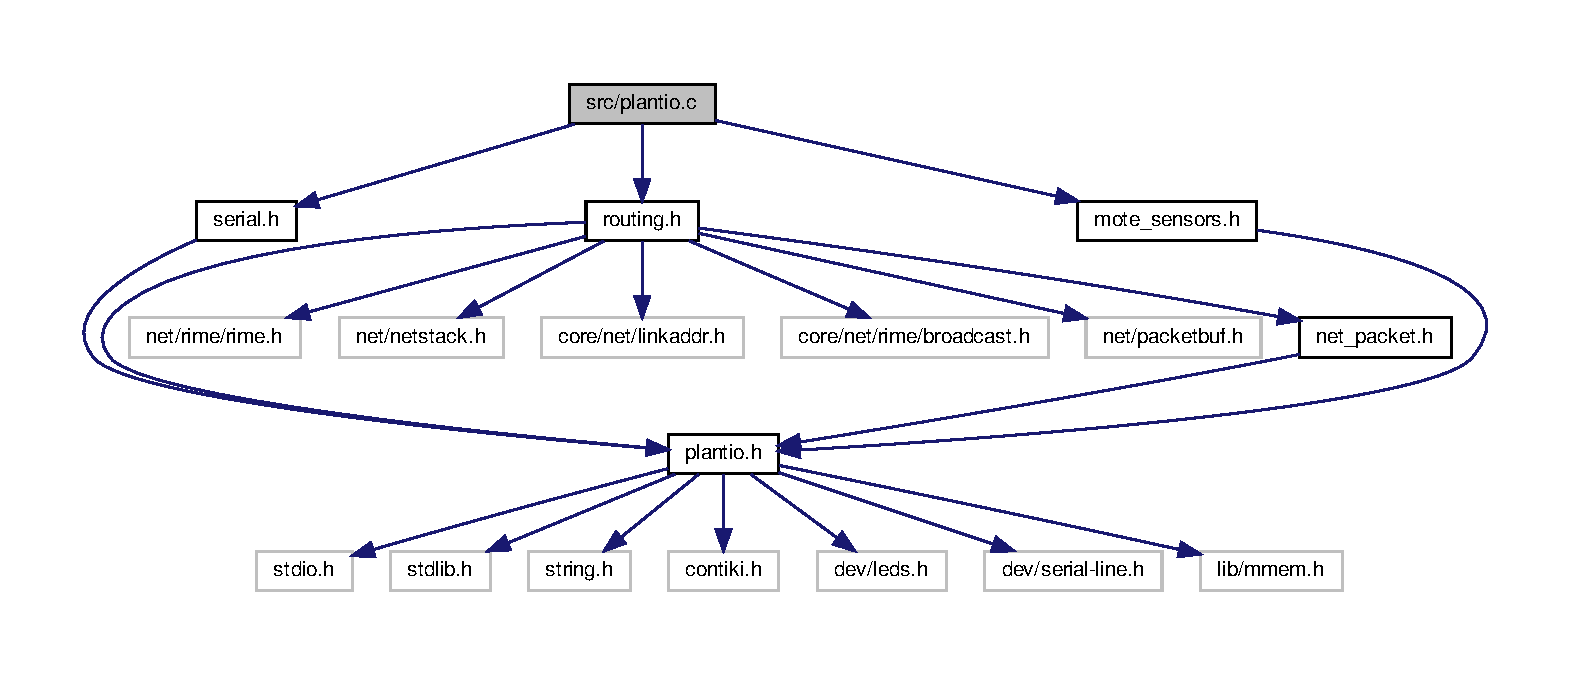
\includegraphics[width=350pt]{plantio_8c__incl}
\end{center}
\end{figure}
\subsection*{Functions}
\begin{DoxyCompactItemize}
\item 
\mbox{\Hypertarget{plantio_8c_ac4b75e05f419a555807e7972c49ccfa6}\label{plantio_8c_ac4b75e05f419a555807e7972c49ccfa6}} 
{\bfseries P\+R\+O\+C\+E\+SS} (p\+\_\+main, \char`\"{}Main process\char`\"{})
\item 
\mbox{\Hypertarget{plantio_8c_a748a4b425bfc98c0a99519ec565d6846}\label{plantio_8c_a748a4b425bfc98c0a99519ec565d6846}} 
{\bfseries P\+R\+O\+C\+E\+S\+S\+\_\+\+T\+H\+R\+E\+AD} (p\+\_\+main, ev, data)
\end{DoxyCompactItemize}
\subsection*{Variables}
\begin{DoxyCompactItemize}
\item 
\mbox{\Hypertarget{plantio_8c_a2c73c0f16ac86b4e8eb2ba48da0cecce}\label{plantio_8c_a2c73c0f16ac86b4e8eb2ba48da0cecce}} 
A\+U\+T\+O\+S\+T\+A\+R\+T\+\_\+\+P\+R\+O\+C\+E\+S\+S\+ES \& {\bfseries p\+\_\+main}
\end{DoxyCompactItemize}


\subsection{Detailed Description}
\begin{DoxyAuthor}{Author}
Patrick Willner (\href{mailto:patrick.willner@tum.de}{\tt patrick.\+willner@tum.\+de}), Andreas Koliopoulos (\href{mailto:ga96leh@mytum.de}{\tt ga96leh@mytum.\+de}), Alexander Schmaus (\href{mailto:ga96fin@mytum.de}{\tt ga96fin@mytum.\+de}) 
\end{DoxyAuthor}
\begin{DoxyVersion}{Version}
0.\+1 
\end{DoxyVersion}
\begin{DoxyDate}{Date}
2019-\/12-\/14
\end{DoxyDate}
\begin{DoxyCopyright}{Copyright}
Copyright (c) 2019 
\end{DoxyCopyright}

\hypertarget{plantio_8h}{}\section{src/plantio.h File Reference}
\label{plantio_8h}\index{src/plantio.\+h@{src/plantio.\+h}}
{\ttfamily \#include $<$stdio.\+h$>$}\newline
{\ttfamily \#include $<$stdlib.\+h$>$}\newline
{\ttfamily \#include $<$string.\+h$>$}\newline
{\ttfamily \#include $<$contiki.\+h$>$}\newline
{\ttfamily \#include $<$dev/leds.\+h$>$}\newline
{\ttfamily \#include $<$dev/serial-\/line.\+h$>$}\newline
{\ttfamily \#include $<$lib/mmem.\+h$>$}\newline
Include dependency graph for plantio.\+h\+:\nopagebreak
\begin{figure}[H]
\begin{center}
\leavevmode
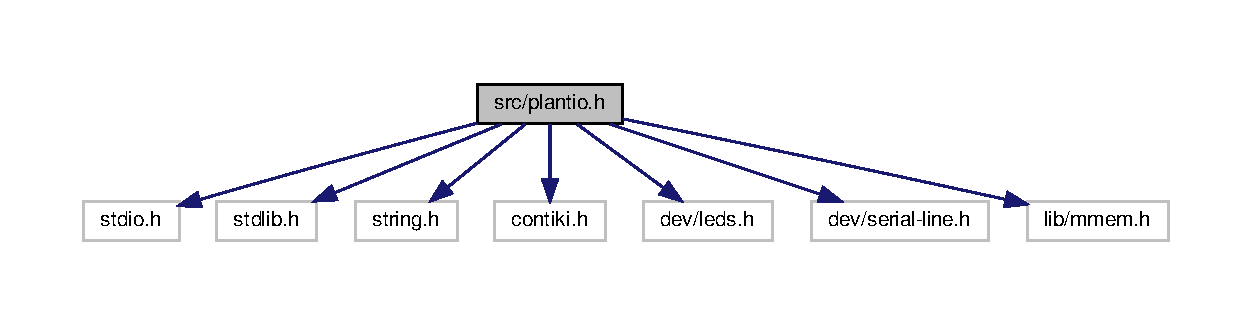
\includegraphics[width=350pt]{plantio_8h__incl}
\end{center}
\end{figure}
This graph shows which files directly or indirectly include this file\+:\nopagebreak
\begin{figure}[H]
\begin{center}
\leavevmode
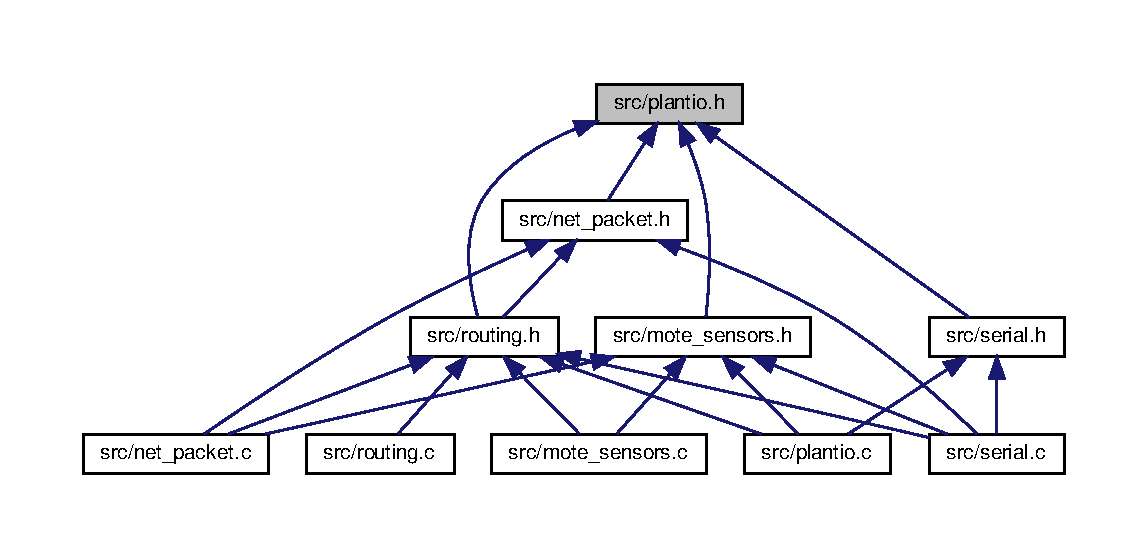
\includegraphics[width=350pt]{plantio_8h__dep__incl}
\end{center}
\end{figure}
\subsection*{Macros}
\begin{DoxyCompactItemize}
\item 
\mbox{\Hypertarget{plantio_8h_a6224ffcbd53b35ff382a4ea1b3d613d1}\label{plantio_8h_a6224ffcbd53b35ff382a4ea1b3d613d1}} 
\#define {\bfseries P\+A\+C\+K\+E\+T\+B\+U\+F\+\_\+\+C\+O\+N\+F\+\_\+\+S\+I\+ZE}~256
\item 
\#define \hyperlink{plantio_8h_ad38f3f58cc4e8d2509dec1b398cfed14}{P\+L\+A\+N\+T\+I\+O\+\_\+\+M\+I\+N\+\_\+\+R\+S\+SI}~-\/60
\begin{DoxyCompactList}\small\item\em Defines the R\+S\+SI threshold. \end{DoxyCompactList}\item 
\mbox{\Hypertarget{plantio_8h_af80fa184adf551500f54b2cfaa9ddd95}\label{plantio_8h_af80fa184adf551500f54b2cfaa9ddd95}} 
\#define \hyperlink{plantio_8h_af80fa184adf551500f54b2cfaa9ddd95}{P\+L\+A\+N\+T\+I\+O\+\_\+\+R\+R\+E\+P\+\_\+\+T\+I\+M\+E\+O\+UT}~3
\begin{DoxyCompactList}\small\item\em Defines the default timeout in seconds before a node transmits its best route to the G\+UI. \end{DoxyCompactList}\item 
\mbox{\Hypertarget{plantio_8h_a2e8519190d74767703e56ba914be740e}\label{plantio_8h_a2e8519190d74767703e56ba914be740e}} 
\#define \hyperlink{plantio_8h_a2e8519190d74767703e56ba914be740e}{M\+A\+X\+\_\+\+N\+U\+M\+\_\+\+O\+F\+\_\+\+V\+A\+L\+U\+ES}~10
\begin{DoxyCompactList}\small\item\em Defines the maximum number of sensors data values to be stored. \end{DoxyCompactList}\item 
\mbox{\Hypertarget{plantio_8h_acf88b2723d705d90dd1008f45db2ee68}\label{plantio_8h_acf88b2723d705d90dd1008f45db2ee68}} 
\#define {\bfseries F\+I\+L\+E\+\_\+\+S\+E\+N\+S\+O\+RS}~\char`\"{}fsensors\char`\"{}
\item 
\mbox{\Hypertarget{plantio_8h_a5f4acbdc64328f4665b7231052802ba4}\label{plantio_8h_a5f4acbdc64328f4665b7231052802ba4}} 
\#define {\bfseries F\+I\+L\+E\+\_\+\+R\+O\+U\+T\+I\+NG}~\char`\"{}frouting\char`\"{}
\item 
\#define \hyperlink{plantio_8h_aeedc188900bf33cd14220d4b4a5fb6f7}{plantio\+\_\+malloc}(managed\+\_\+memory,  T,  varname,  size)
\begin{DoxyCompactList}\small\item\em Macro for allocating dynamic memory. \end{DoxyCompactList}\item 
\#define \hyperlink{plantio_8h_ac163b07d4bd02ed21b9b76c310d2a2f2}{plantio\+\_\+free}(managed\+\_\+memory)~mmem\+\_\+free(\&managed\+\_\+memory)
\begin{DoxyCompactList}\small\item\em Frees the dynamic allocated memory. \end{DoxyCompactList}\end{DoxyCompactItemize}
\subsection*{Enumerations}
\begin{DoxyCompactItemize}
\item 
\mbox{\Hypertarget{plantio_8h_aedfc9d8254f442cb95c1b5784835ef9b}\label{plantio_8h_aedfc9d8254f442cb95c1b5784835ef9b}} 
enum \hyperlink{plantio_8h_aedfc9d8254f442cb95c1b5784835ef9b}{thresh} \{ \newline
{\bfseries T\+E\+M\+P\+\_\+\+L\+OW}, 
{\bfseries T\+E\+M\+P\+\_\+\+H\+I\+GH}, 
{\bfseries H\+U\+M\+\_\+\+L\+OW}, 
{\bfseries H\+U\+M\+\_\+\+H\+I\+GH}, 
\newline
{\bfseries L\+I\+G\+H\+T\+\_\+\+L\+OW}, 
{\bfseries L\+I\+G\+H\+T\+\_\+\+H\+I\+GH}
 \}\begin{DoxyCompactList}\small\item\em Defines I\+Ds for different Thresholds. \end{DoxyCompactList}
\end{DoxyCompactItemize}


\subsection{Detailed Description}
\begin{DoxyAuthor}{Author}
Patrick Willner (\href{mailto:patrick.willner@tum.de}{\tt patrick.\+willner@tum.\+de}), Andreas Koliopoulos (\href{mailto:ga96leh@mytum.de}{\tt ga96leh@mytum.\+de}), Alexander Schmaus (\href{mailto:ga96fin@mytum.de}{\tt ga96fin@mytum.\+de}) 
\end{DoxyAuthor}
\begin{DoxyVersion}{Version}
0.\+1 
\end{DoxyVersion}
\begin{DoxyDate}{Date}
2019-\/12-\/14
\end{DoxyDate}
\begin{DoxyCopyright}{Copyright}
Copyright (c) 2019 
\end{DoxyCopyright}


\subsection{Macro Definition Documentation}
\mbox{\Hypertarget{plantio_8h_ac163b07d4bd02ed21b9b76c310d2a2f2}\label{plantio_8h_ac163b07d4bd02ed21b9b76c310d2a2f2}} 
\index{plantio.\+h@{plantio.\+h}!plantio\+\_\+free@{plantio\+\_\+free}}
\index{plantio\+\_\+free@{plantio\+\_\+free}!plantio.\+h@{plantio.\+h}}
\subsubsection{\texorpdfstring{plantio\+\_\+free}{plantio\_free}}
{\footnotesize\ttfamily \#define plantio\+\_\+free(\begin{DoxyParamCaption}\item[{}]{managed\+\_\+memory }\end{DoxyParamCaption})~mmem\+\_\+free(\&managed\+\_\+memory)}



Frees the dynamic allocated memory. 


\begin{DoxyParams}{Parameters}
{\em managed\+\_\+memory} & Managed memory struct instance name \\
\hline
\end{DoxyParams}
\mbox{\Hypertarget{plantio_8h_aeedc188900bf33cd14220d4b4a5fb6f7}\label{plantio_8h_aeedc188900bf33cd14220d4b4a5fb6f7}} 
\index{plantio.\+h@{plantio.\+h}!plantio\+\_\+malloc@{plantio\+\_\+malloc}}
\index{plantio\+\_\+malloc@{plantio\+\_\+malloc}!plantio.\+h@{plantio.\+h}}
\subsubsection{\texorpdfstring{plantio\+\_\+malloc}{plantio\_malloc}}
{\footnotesize\ttfamily \#define plantio\+\_\+malloc(\begin{DoxyParamCaption}\item[{}]{managed\+\_\+memory,  }\item[{}]{T,  }\item[{}]{varname,  }\item[{}]{size }\end{DoxyParamCaption})}

{\bfseries Value\+:}
\begin{DoxyCode}
\textcolor{keyword}{struct }mmem managed\_memory;                          \(\backslash\)
    mmem\_alloc(&managed\_memory, size);                   \(\backslash\)
    T *varname = (T *)((\textcolor{keyword}{struct} mmem *)(&managed\_memory)->ptr)
\end{DoxyCode}


Macro for allocating dynamic memory. 

Uses the contiki managed memory library.


\begin{DoxyParams}{Parameters}
{\em managed\+\_\+memory} & Managed memory struct instance name \\
\hline
{\em T} & Datatype to be allocated \\
\hline
{\em varname} & Name of the pointer to T \\
\hline
{\em size} & Size of allocated memory \\
\hline
\end{DoxyParams}
\mbox{\Hypertarget{plantio_8h_ad38f3f58cc4e8d2509dec1b398cfed14}\label{plantio_8h_ad38f3f58cc4e8d2509dec1b398cfed14}} 
\index{plantio.\+h@{plantio.\+h}!P\+L\+A\+N\+T\+I\+O\+\_\+\+M\+I\+N\+\_\+\+R\+S\+SI@{P\+L\+A\+N\+T\+I\+O\+\_\+\+M\+I\+N\+\_\+\+R\+S\+SI}}
\index{P\+L\+A\+N\+T\+I\+O\+\_\+\+M\+I\+N\+\_\+\+R\+S\+SI@{P\+L\+A\+N\+T\+I\+O\+\_\+\+M\+I\+N\+\_\+\+R\+S\+SI}!plantio.\+h@{plantio.\+h}}
\subsubsection{\texorpdfstring{P\+L\+A\+N\+T\+I\+O\+\_\+\+M\+I\+N\+\_\+\+R\+S\+SI}{PLANTIO\_MIN\_RSSI}}
{\footnotesize\ttfamily \#define P\+L\+A\+N\+T\+I\+O\+\_\+\+M\+I\+N\+\_\+\+R\+S\+SI~-\/60}



Defines the R\+S\+SI threshold. 

Broadcast packets below this thresholds are dropped. 
\hypertarget{routing_8c}{}\section{src/routing.c File Reference}
\label{routing_8c}\index{src/routing.\+c@{src/routing.\+c}}
{\ttfamily \#include \char`\"{}routing.\+h\char`\"{}}\newline
{\ttfamily \#include \char`\"{}cfs/cfs.\+h\char`\"{}}\newline
{\ttfamily \#include \char`\"{}sys/etimer.\+h\char`\"{}}\newline
{\ttfamily \#include \char`\"{}random.\+h\char`\"{}}\newline
{\ttfamily \#include \char`\"{}clock.\+h\char`\"{}}\newline
Include dependency graph for routing.\+c\+:
\nopagebreak
\begin{figure}[H]
\begin{center}
\leavevmode
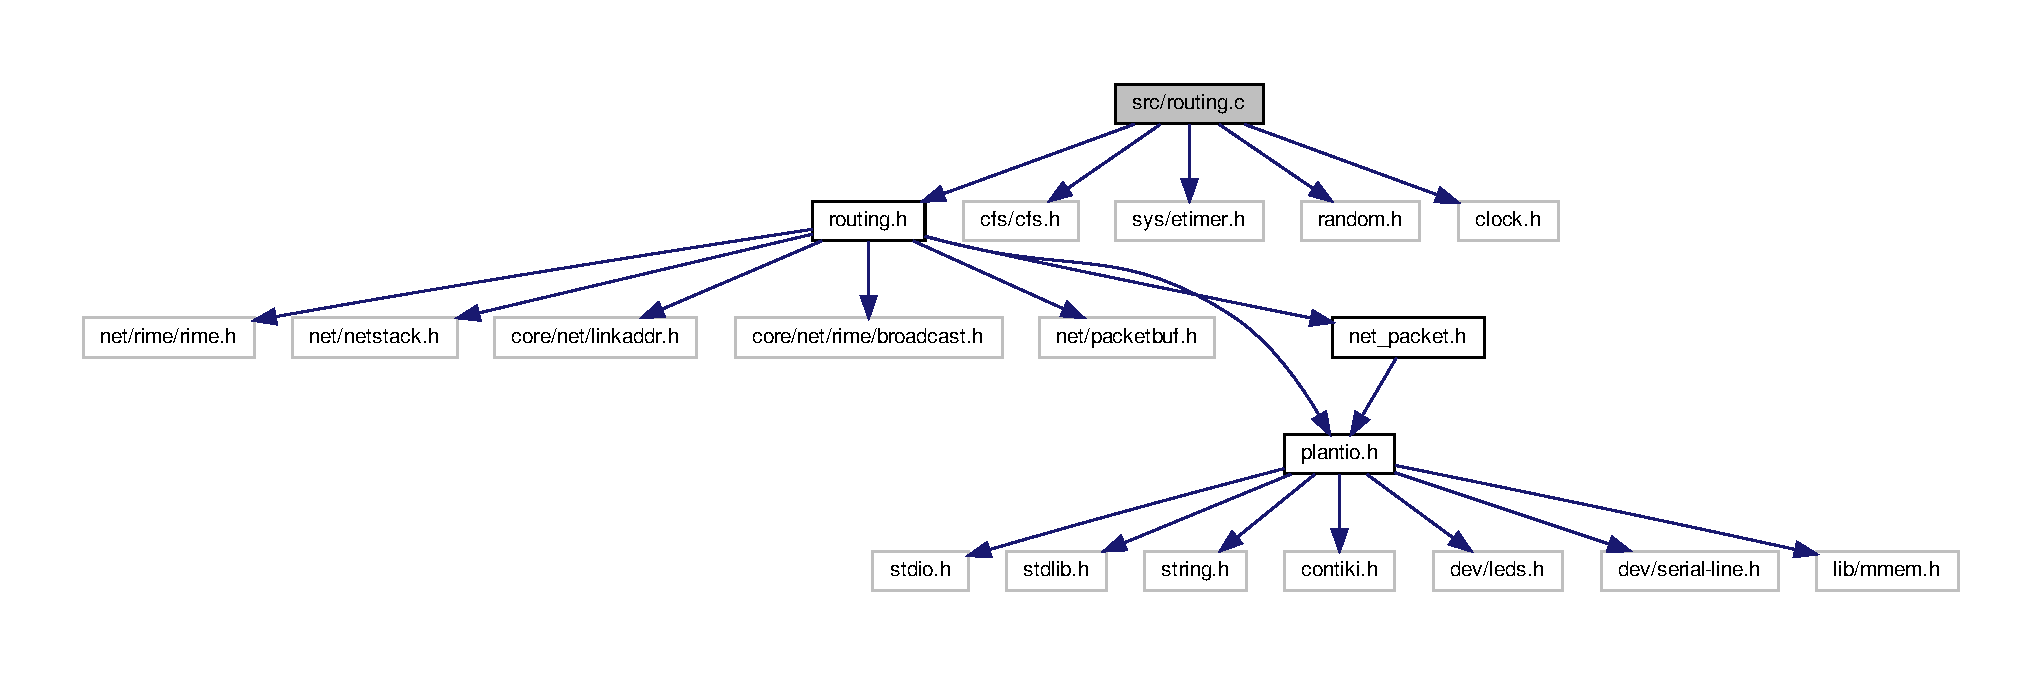
\includegraphics[width=350pt]{routing_8c__incl}
\end{center}
\end{figure}
\subsection*{Functions}
\begin{DoxyCompactItemize}
\item 
\mbox{\Hypertarget{routing_8c_ae2d190e672275a545b4de4c3cd6b32b0}\label{routing_8c_ae2d190e672275a545b4de4c3cd6b32b0}} 
{\bfseries P\+R\+O\+C\+E\+SS} (\hyperlink{routing_8h_a5a6576fde225bfed1b06f8cf761bcb84}{p\+\_\+conn}, \char`\"{}\char`\"{})
\item 
\mbox{\Hypertarget{routing_8c_adf5d30ba729719a7b1ea6d22ab35c9b9}\label{routing_8c_adf5d30ba729719a7b1ea6d22ab35c9b9}} 
{\bfseries P\+R\+O\+C\+E\+S\+S\+\_\+\+T\+H\+R\+E\+AD} (\hyperlink{routing_8h_a5a6576fde225bfed1b06f8cf761bcb84}{p\+\_\+conn}, ev, data)
\item 
\mbox{\Hypertarget{routing_8c_a0bc30dd58e5e0c26ada4b8b94447d132}\label{routing_8c_a0bc30dd58e5e0c26ada4b8b94447d132}} 
{\bfseries P\+R\+O\+C\+E\+SS} (\hyperlink{routing_8h_a4c12d3f6cf50b4f1de83cb9702365575}{p\+\_\+init\+\_\+reply\+\_\+timer}, \char`\"{}\char`\"{})
\item 
\mbox{\Hypertarget{routing_8c_af0605f4fed483775266bc7855e0b2270}\label{routing_8c_af0605f4fed483775266bc7855e0b2270}} 
{\bfseries P\+R\+O\+C\+E\+S\+S\+\_\+\+T\+H\+R\+E\+AD} (\hyperlink{routing_8h_a4c12d3f6cf50b4f1de83cb9702365575}{p\+\_\+init\+\_\+reply\+\_\+timer}, ev, data)
\item 
void \hyperlink{routing_8c_a13eb496f6046eac861006b61d60dc196}{broadcast\+\_\+receive} (struct broadcast\+\_\+conn $\ast$broadcast, const linkaddr\+\_\+t $\ast$from)
\begin{DoxyCompactList}\small\item\em Callback function for Broadcast. \end{DoxyCompactList}\item 
void \hyperlink{routing_8c_a8a3474e4cd76194d0eb2ac744eda8c7c}{unicast\+\_\+receive} (struct unicast\+\_\+conn $\ast$unicast, const linkaddr\+\_\+t $\ast$from)
\begin{DoxyCompactList}\small\item\em Callback function for Unicast. \end{DoxyCompactList}\item 
void \hyperlink{routing_8c_aa8cb8a8be4c104f1b1405ed682f8e191}{init\+\_\+network} (void)
\begin{DoxyCompactList}\small\item\em Starts the network discovery algorithm. \end{DoxyCompactList}\item 
void \hyperlink{routing_8c_a20f9e50ac25cd018884fec58b70b13a5}{forward\+\_\+discover} (const plantio\+\_\+packet\+\_\+t $\ast$packet)
\begin{DoxyCompactList}\small\item\em Forwards the network discovery packet \& updates the routing tables. \end{DoxyCompactList}\item 
\mbox{\Hypertarget{routing_8c_a52613d7923f35868e7e0dd3e7f2e47dc}\label{routing_8c_a52613d7923f35868e7e0dd3e7f2e47dc}} 
void \hyperlink{routing_8c_a52613d7923f35868e7e0dd3e7f2e47dc}{find\+\_\+best\+\_\+route} (void)
\begin{DoxyCompactList}\small\item\em Finds the optimal route in the routing table by minimizing the number of hops. \end{DoxyCompactList}\item 
const int16\+\_\+t \hyperlink{routing_8c_a605aa3d917cc42b30dd2ed242970a195}{get\+\_\+best\+\_\+route\+\_\+index} (void)
\begin{DoxyCompactList}\small\item\em Get the index of the optimal route in the routing table. -\/1 if table is empty or the current node is the G\+UI node. \end{DoxyCompactList}\item 
\mbox{\Hypertarget{routing_8c_a033ff0c93dd6d1991c523d4466992332}\label{routing_8c_a033ff0c93dd6d1991c523d4466992332}} 
void \hyperlink{routing_8c_a033ff0c93dd6d1991c523d4466992332}{print\+\_\+routing\+\_\+table} (void)
\begin{DoxyCompactList}\small\item\em Prints the routing table. \end{DoxyCompactList}\item 
\mbox{\Hypertarget{routing_8c_a6c7443691d2e4c92e28dc8e13f18fb82}\label{routing_8c_a6c7443691d2e4c92e28dc8e13f18fb82}} 
void \hyperlink{routing_8c_a6c7443691d2e4c92e28dc8e13f18fb82}{clear\+\_\+routing\+\_\+table} (void)
\begin{DoxyCompactList}\small\item\em Clears the routing table. \end{DoxyCompactList}\item 
void \hyperlink{routing_8c_a10c2716d53419a0ec9111c644904c9b9}{write\+\_\+routing\+\_\+table} (const uint8\+\_\+t $\ast$route, const uint8\+\_\+t length)
\begin{DoxyCompactList}\small\item\em Write a route to the routing table on the flash memory. \end{DoxyCompactList}\item 
const uint16\+\_\+t \hyperlink{routing_8c_a5b87ed069c6951f8d390154609c487c0}{get\+\_\+num\+\_\+routes} (void)
\begin{DoxyCompactList}\small\item\em Get the number of entries in the routing table. \end{DoxyCompactList}\item 
const uint8\+\_\+t \hyperlink{routing_8c_a4b6ac79ba38213a3f4390d5d3a9fb095}{get\+\_\+num\+\_\+hops} (const uint16\+\_\+t index)
\begin{DoxyCompactList}\small\item\em Get the number of hops for a route with given index in the routing table. \end{DoxyCompactList}\item 
void \hyperlink{routing_8c_a4530e9af1504c8a4cf003a3ad4abf818}{get\+\_\+route} (uint8\+\_\+t $\ast$route, const uint16\+\_\+t num\+\_\+hops, const uint16\+\_\+t index)
\begin{DoxyCompactList}\small\item\em Get the route for given index in the routing table. \end{DoxyCompactList}\item 
\mbox{\Hypertarget{routing_8c_ac41726b09440e72c5cc9dee53fc13aec}\label{routing_8c_ac41726b09440e72c5cc9dee53fc13aec}} 
void \hyperlink{routing_8c_ac41726b09440e72c5cc9dee53fc13aec}{init\+\_\+rreq\+\_\+reply} (const uint16\+\_\+t index)
\begin{DoxyCompactList}\small\item\em Selects the optimal route to the G\+UI node and transmits it to the G\+UI node. \end{DoxyCompactList}\item 
void \hyperlink{routing_8c_a3639eb60506758c56bbc601911a71c64}{forward\+\_\+routing} (const plantio\+\_\+packet\+\_\+t $\ast$packet)
\begin{DoxyCompactList}\small\item\em Updates the Source and Destionation of incoming packets and forwards the packet to the next hop if necessary. \end{DoxyCompactList}\item 
void \hyperlink{routing_8c_a8724d80f3f41082d62dbaad8f6ebeedf}{init\+\_\+data\+\_\+packet} (const uint8\+\_\+t type, const uint8\+\_\+t dest, const uint8\+\_\+t $\ast$data, const uint8\+\_\+t data\+\_\+len, int index)
\begin{DoxyCompactList}\small\item\em Sends a data packet (id $>$= 10) to any node in the network. \end{DoxyCompactList}\item 
void \hyperlink{routing_8c_ab97d23714b07247e89e011908d6fafcc}{add\+\_\+device\+\_\+to\+\_\+network} (void)
\begin{DoxyCompactList}\small\item\em Add the current node to an existing network. \end{DoxyCompactList}\item 
void \hyperlink{routing_8c_a2b3ed1fa69f729b9eaeeae3357ed4648}{send\+\_\+best\+\_\+route} (const uint8\+\_\+t dest)
\begin{DoxyCompactList}\small\item\em Sends the best route of current device to the destination via unicast. \end{DoxyCompactList}\item 
void \hyperlink{routing_8c_a0a32fd3503c9d77a6bfb62a66f3e47e1}{receive\+\_\+route} (const plantio\+\_\+packet\+\_\+t $\ast$packet)
\begin{DoxyCompactList}\small\item\em Saves the route in the routing table, starts a timer and schedules an R\+R\+EP to the G\+UI node with the best route. \end{DoxyCompactList}\item 
void \hyperlink{routing_8c_ac960ae2b0934e5ce84cd3cc822eb69be}{send\+\_\+ack} (const uint8\+\_\+t $\ast$route, const uint8\+\_\+t len)
\begin{DoxyCompactList}\small\item\em Sends an A\+CK Packet via the given route. \end{DoxyCompactList}\end{DoxyCompactItemize}


\subsection{Detailed Description}
\begin{DoxyAuthor}{Author}
Patrick Willner (\href{mailto:patrick.willner@tum.de}{\tt patrick.\+willner@tum.\+de}), Andreas Koliopoulos (\href{mailto:ga96leh@mytum.de}{\tt ga96leh@mytum.\+de}), Alexander Schmaus (\href{mailto:ga96fin@mytum.de}{\tt ga96fin@mytum.\+de}) 
\end{DoxyAuthor}
\begin{DoxyVersion}{Version}
0.\+1 
\end{DoxyVersion}
\begin{DoxyDate}{Date}
2019-\/12-\/12
\end{DoxyDate}
\begin{DoxyCopyright}{Copyright}
Copyright (c) 2019 
\end{DoxyCopyright}


\subsection{Function Documentation}
\mbox{\Hypertarget{routing_8c_ab97d23714b07247e89e011908d6fafcc}\label{routing_8c_ab97d23714b07247e89e011908d6fafcc}} 
\index{routing.\+c@{routing.\+c}!add\+\_\+device\+\_\+to\+\_\+network@{add\+\_\+device\+\_\+to\+\_\+network}}
\index{add\+\_\+device\+\_\+to\+\_\+network@{add\+\_\+device\+\_\+to\+\_\+network}!routing.\+c@{routing.\+c}}
\subsubsection{\texorpdfstring{add\+\_\+device\+\_\+to\+\_\+network()}{add\_device\_to\_network()}}
{\footnotesize\ttfamily void add\+\_\+device\+\_\+to\+\_\+network (\begin{DoxyParamCaption}\item[{void}]{ }\end{DoxyParamCaption})}



Add the current node to an existing network. 

Starts a broadcast to neighbouring nodes which then reply with their best route to the G\+UI node. \mbox{\Hypertarget{routing_8c_a13eb496f6046eac861006b61d60dc196}\label{routing_8c_a13eb496f6046eac861006b61d60dc196}} 
\index{routing.\+c@{routing.\+c}!broadcast\+\_\+receive@{broadcast\+\_\+receive}}
\index{broadcast\+\_\+receive@{broadcast\+\_\+receive}!routing.\+c@{routing.\+c}}
\subsubsection{\texorpdfstring{broadcast\+\_\+receive()}{broadcast\_receive()}}
{\footnotesize\ttfamily void broadcast\+\_\+receive (\begin{DoxyParamCaption}\item[{struct broadcast\+\_\+conn $\ast$}]{broadcast,  }\item[{const linkaddr\+\_\+t $\ast$}]{from }\end{DoxyParamCaption})}



Callback function for Broadcast. 


\begin{DoxyParams}{Parameters}
{\em broadcast} & Broadcast Connection \\
\hline
{\em from} & Node ID of packet source \\
\hline
\end{DoxyParams}
\mbox{\Hypertarget{routing_8c_a20f9e50ac25cd018884fec58b70b13a5}\label{routing_8c_a20f9e50ac25cd018884fec58b70b13a5}} 
\index{routing.\+c@{routing.\+c}!forward\+\_\+discover@{forward\+\_\+discover}}
\index{forward\+\_\+discover@{forward\+\_\+discover}!routing.\+c@{routing.\+c}}
\subsubsection{\texorpdfstring{forward\+\_\+discover()}{forward\_discover()}}
{\footnotesize\ttfamily void forward\+\_\+discover (\begin{DoxyParamCaption}\item[{const plantio\+\_\+packet\+\_\+t $\ast$}]{packet }\end{DoxyParamCaption})}



Forwards the network discovery packet \& updates the routing tables. 

Packets with current Node ID in the source as well as transmissions below P\+L\+A\+N\+T\+I\+O\+\_\+\+M\+I\+N\+\_\+\+R\+S\+SI threshold will be dropped.


\begin{DoxyParams}{Parameters}
{\em packet} & Pointer to instance of plantio\+\_\+packet\+\_\+t \\
\hline
\end{DoxyParams}
\mbox{\Hypertarget{routing_8c_a3639eb60506758c56bbc601911a71c64}\label{routing_8c_a3639eb60506758c56bbc601911a71c64}} 
\index{routing.\+c@{routing.\+c}!forward\+\_\+routing@{forward\+\_\+routing}}
\index{forward\+\_\+routing@{forward\+\_\+routing}!routing.\+c@{routing.\+c}}
\subsubsection{\texorpdfstring{forward\+\_\+routing()}{forward\_routing()}}
{\footnotesize\ttfamily void forward\+\_\+routing (\begin{DoxyParamCaption}\item[{const plantio\+\_\+packet\+\_\+t $\ast$}]{packet }\end{DoxyParamCaption})}



Updates the Source and Destionation of incoming packets and forwards the packet to the next hop if necessary. 


\begin{DoxyParams}{Parameters}
{\em packet} & Instance of packet struct \\
\hline
\end{DoxyParams}
\mbox{\Hypertarget{routing_8c_a605aa3d917cc42b30dd2ed242970a195}\label{routing_8c_a605aa3d917cc42b30dd2ed242970a195}} 
\index{routing.\+c@{routing.\+c}!get\+\_\+best\+\_\+route\+\_\+index@{get\+\_\+best\+\_\+route\+\_\+index}}
\index{get\+\_\+best\+\_\+route\+\_\+index@{get\+\_\+best\+\_\+route\+\_\+index}!routing.\+c@{routing.\+c}}
\subsubsection{\texorpdfstring{get\+\_\+best\+\_\+route\+\_\+index()}{get\_best\_route\_index()}}
{\footnotesize\ttfamily const int16\+\_\+t get\+\_\+best\+\_\+route\+\_\+index (\begin{DoxyParamCaption}\item[{void}]{ }\end{DoxyParamCaption})}



Get the index of the optimal route in the routing table. -\/1 if table is empty or the current node is the G\+UI node. 

\begin{DoxyReturn}{Returns}
const int16\+\_\+t Index of route in the routing table 
\end{DoxyReturn}
\mbox{\Hypertarget{routing_8c_a4b6ac79ba38213a3f4390d5d3a9fb095}\label{routing_8c_a4b6ac79ba38213a3f4390d5d3a9fb095}} 
\index{routing.\+c@{routing.\+c}!get\+\_\+num\+\_\+hops@{get\+\_\+num\+\_\+hops}}
\index{get\+\_\+num\+\_\+hops@{get\+\_\+num\+\_\+hops}!routing.\+c@{routing.\+c}}
\subsubsection{\texorpdfstring{get\+\_\+num\+\_\+hops()}{get\_num\_hops()}}
{\footnotesize\ttfamily const uint8\+\_\+t get\+\_\+num\+\_\+hops (\begin{DoxyParamCaption}\item[{const uint16\+\_\+t}]{index }\end{DoxyParamCaption})}



Get the number of hops for a route with given index in the routing table. 


\begin{DoxyParams}{Parameters}
{\em index} & Index of route in table \\
\hline
\end{DoxyParams}
\begin{DoxyReturn}{Returns}
const uint16\+\_\+t Number of hops 
\end{DoxyReturn}
\mbox{\Hypertarget{routing_8c_a5b87ed069c6951f8d390154609c487c0}\label{routing_8c_a5b87ed069c6951f8d390154609c487c0}} 
\index{routing.\+c@{routing.\+c}!get\+\_\+num\+\_\+routes@{get\+\_\+num\+\_\+routes}}
\index{get\+\_\+num\+\_\+routes@{get\+\_\+num\+\_\+routes}!routing.\+c@{routing.\+c}}
\subsubsection{\texorpdfstring{get\+\_\+num\+\_\+routes()}{get\_num\_routes()}}
{\footnotesize\ttfamily const uint16\+\_\+t get\+\_\+num\+\_\+routes (\begin{DoxyParamCaption}\item[{void}]{ }\end{DoxyParamCaption})}



Get the number of entries in the routing table. 

\begin{DoxyReturn}{Returns}
const uint16\+\_\+t Number of routes 
\end{DoxyReturn}
\mbox{\Hypertarget{routing_8c_a4530e9af1504c8a4cf003a3ad4abf818}\label{routing_8c_a4530e9af1504c8a4cf003a3ad4abf818}} 
\index{routing.\+c@{routing.\+c}!get\+\_\+route@{get\+\_\+route}}
\index{get\+\_\+route@{get\+\_\+route}!routing.\+c@{routing.\+c}}
\subsubsection{\texorpdfstring{get\+\_\+route()}{get\_route()}}
{\footnotesize\ttfamily void get\+\_\+route (\begin{DoxyParamCaption}\item[{uint8\+\_\+t $\ast$}]{route,  }\item[{const uint16\+\_\+t}]{num\+\_\+hops,  }\item[{const uint16\+\_\+t}]{index }\end{DoxyParamCaption})}



Get the route for given index in the routing table. 


\begin{DoxyParams}{Parameters}
{\em route} & Pointer to the allocated memory for the route \\
\hline
{\em num\+\_\+hops} & Number of hops \\
\hline
{\em index} & Index of route in table \\
\hline
\end{DoxyParams}
\mbox{\Hypertarget{routing_8c_a8724d80f3f41082d62dbaad8f6ebeedf}\label{routing_8c_a8724d80f3f41082d62dbaad8f6ebeedf}} 
\index{routing.\+c@{routing.\+c}!init\+\_\+data\+\_\+packet@{init\+\_\+data\+\_\+packet}}
\index{init\+\_\+data\+\_\+packet@{init\+\_\+data\+\_\+packet}!routing.\+c@{routing.\+c}}
\subsubsection{\texorpdfstring{init\+\_\+data\+\_\+packet()}{init\_data\_packet()}}
{\footnotesize\ttfamily void init\+\_\+data\+\_\+packet (\begin{DoxyParamCaption}\item[{const uint8\+\_\+t}]{type,  }\item[{const uint8\+\_\+t}]{dest,  }\item[{const uint8\+\_\+t $\ast$}]{data,  }\item[{const uint8\+\_\+t}]{data\+\_\+len,  }\item[{int}]{index }\end{DoxyParamCaption})}



Sends a data packet (id $>$= 10) to any node in the network. 


\begin{DoxyParams}{Parameters}
{\em type} & Type of packet \\
\hline
{\em dest} & Destination node id \\
\hline
{\em data} & Pointer to byte array data \\
\hline
{\em data\+\_\+len} & Data length \\
\hline
{\em index} & Index of route in table, set to -\/1 if not known \\
\hline
\end{DoxyParams}
\mbox{\Hypertarget{routing_8c_aa8cb8a8be4c104f1b1405ed682f8e191}\label{routing_8c_aa8cb8a8be4c104f1b1405ed682f8e191}} 
\index{routing.\+c@{routing.\+c}!init\+\_\+network@{init\+\_\+network}}
\index{init\+\_\+network@{init\+\_\+network}!routing.\+c@{routing.\+c}}
\subsubsection{\texorpdfstring{init\+\_\+network()}{init\_network()}}
{\footnotesize\ttfamily void init\+\_\+network (\begin{DoxyParamCaption}\item[{void}]{ }\end{DoxyParamCaption})}



Starts the network discovery algorithm. 

Floods the network with a network discory packet. \mbox{\Hypertarget{routing_8c_a0a32fd3503c9d77a6bfb62a66f3e47e1}\label{routing_8c_a0a32fd3503c9d77a6bfb62a66f3e47e1}} 
\index{routing.\+c@{routing.\+c}!receive\+\_\+route@{receive\+\_\+route}}
\index{receive\+\_\+route@{receive\+\_\+route}!routing.\+c@{routing.\+c}}
\subsubsection{\texorpdfstring{receive\+\_\+route()}{receive\_route()}}
{\footnotesize\ttfamily void receive\+\_\+route (\begin{DoxyParamCaption}\item[{const plantio\+\_\+packet\+\_\+t $\ast$}]{packet }\end{DoxyParamCaption})}



Saves the route in the routing table, starts a timer and schedules an R\+R\+EP to the G\+UI node with the best route. 


\begin{DoxyParams}{Parameters}
{\em packet} & Instance of packet struct \\
\hline
\end{DoxyParams}
\mbox{\Hypertarget{routing_8c_ac960ae2b0934e5ce84cd3cc822eb69be}\label{routing_8c_ac960ae2b0934e5ce84cd3cc822eb69be}} 
\index{routing.\+c@{routing.\+c}!send\+\_\+ack@{send\+\_\+ack}}
\index{send\+\_\+ack@{send\+\_\+ack}!routing.\+c@{routing.\+c}}
\subsubsection{\texorpdfstring{send\+\_\+ack()}{send\_ack()}}
{\footnotesize\ttfamily void send\+\_\+ack (\begin{DoxyParamCaption}\item[{const uint8\+\_\+t $\ast$}]{route,  }\item[{const uint8\+\_\+t}]{len }\end{DoxyParamCaption})}



Sends an A\+CK Packet via the given route. 


\begin{DoxyParams}{Parameters}
{\em route} & Path to the destination node \\
\hline
\end{DoxyParams}
\mbox{\Hypertarget{routing_8c_a2b3ed1fa69f729b9eaeeae3357ed4648}\label{routing_8c_a2b3ed1fa69f729b9eaeeae3357ed4648}} 
\index{routing.\+c@{routing.\+c}!send\+\_\+best\+\_\+route@{send\+\_\+best\+\_\+route}}
\index{send\+\_\+best\+\_\+route@{send\+\_\+best\+\_\+route}!routing.\+c@{routing.\+c}}
\subsubsection{\texorpdfstring{send\+\_\+best\+\_\+route()}{send\_best\_route()}}
{\footnotesize\ttfamily void send\+\_\+best\+\_\+route (\begin{DoxyParamCaption}\item[{const uint8\+\_\+t}]{dest }\end{DoxyParamCaption})}



Sends the best route of current device to the destination via unicast. 


\begin{DoxyParams}{Parameters}
{\em dest} & Node id of destination \\
\hline
\end{DoxyParams}
\mbox{\Hypertarget{routing_8c_a8a3474e4cd76194d0eb2ac744eda8c7c}\label{routing_8c_a8a3474e4cd76194d0eb2ac744eda8c7c}} 
\index{routing.\+c@{routing.\+c}!unicast\+\_\+receive@{unicast\+\_\+receive}}
\index{unicast\+\_\+receive@{unicast\+\_\+receive}!routing.\+c@{routing.\+c}}
\subsubsection{\texorpdfstring{unicast\+\_\+receive()}{unicast\_receive()}}
{\footnotesize\ttfamily void unicast\+\_\+receive (\begin{DoxyParamCaption}\item[{struct unicast\+\_\+conn $\ast$}]{unicast,  }\item[{const linkaddr\+\_\+t $\ast$}]{from }\end{DoxyParamCaption})}



Callback function for Unicast. 


\begin{DoxyParams}{Parameters}
{\em unicast} & Unicast Connection \\
\hline
{\em from} & Node ID of packet source \\
\hline
\end{DoxyParams}
\mbox{\Hypertarget{routing_8c_a10c2716d53419a0ec9111c644904c9b9}\label{routing_8c_a10c2716d53419a0ec9111c644904c9b9}} 
\index{routing.\+c@{routing.\+c}!write\+\_\+routing\+\_\+table@{write\+\_\+routing\+\_\+table}}
\index{write\+\_\+routing\+\_\+table@{write\+\_\+routing\+\_\+table}!routing.\+c@{routing.\+c}}
\subsubsection{\texorpdfstring{write\+\_\+routing\+\_\+table()}{write\_routing\_table()}}
{\footnotesize\ttfamily void write\+\_\+routing\+\_\+table (\begin{DoxyParamCaption}\item[{const uint8\+\_\+t $\ast$}]{route,  }\item[{const uint8\+\_\+t}]{length }\end{DoxyParamCaption})}



Write a route to the routing table on the flash memory. 


\begin{DoxyParams}{Parameters}
{\em route} & Array of Node I\+Ds \\
\hline
{\em length} & Length of the array, i.\+e. the number of hops of the route \\
\hline
\end{DoxyParams}

\hypertarget{routing_8h}{}\section{src/routing.h File Reference}
\label{routing_8h}\index{src/routing.\+h@{src/routing.\+h}}
{\ttfamily \#include $<$net/rime/rime.\+h$>$}\newline
{\ttfamily \#include $<$net/netstack.\+h$>$}\newline
{\ttfamily \#include $<$core/net/linkaddr.\+h$>$}\newline
{\ttfamily \#include $<$core/net/rime/broadcast.\+h$>$}\newline
{\ttfamily \#include $<$net/packetbuf.\+h$>$}\newline
{\ttfamily \#include \char`\"{}plantio.\+h\char`\"{}}\newline
{\ttfamily \#include \char`\"{}net\+\_\+packet.\+h\char`\"{}}\newline
Include dependency graph for routing.\+h\+:
\nopagebreak
\begin{figure}[H]
\begin{center}
\leavevmode
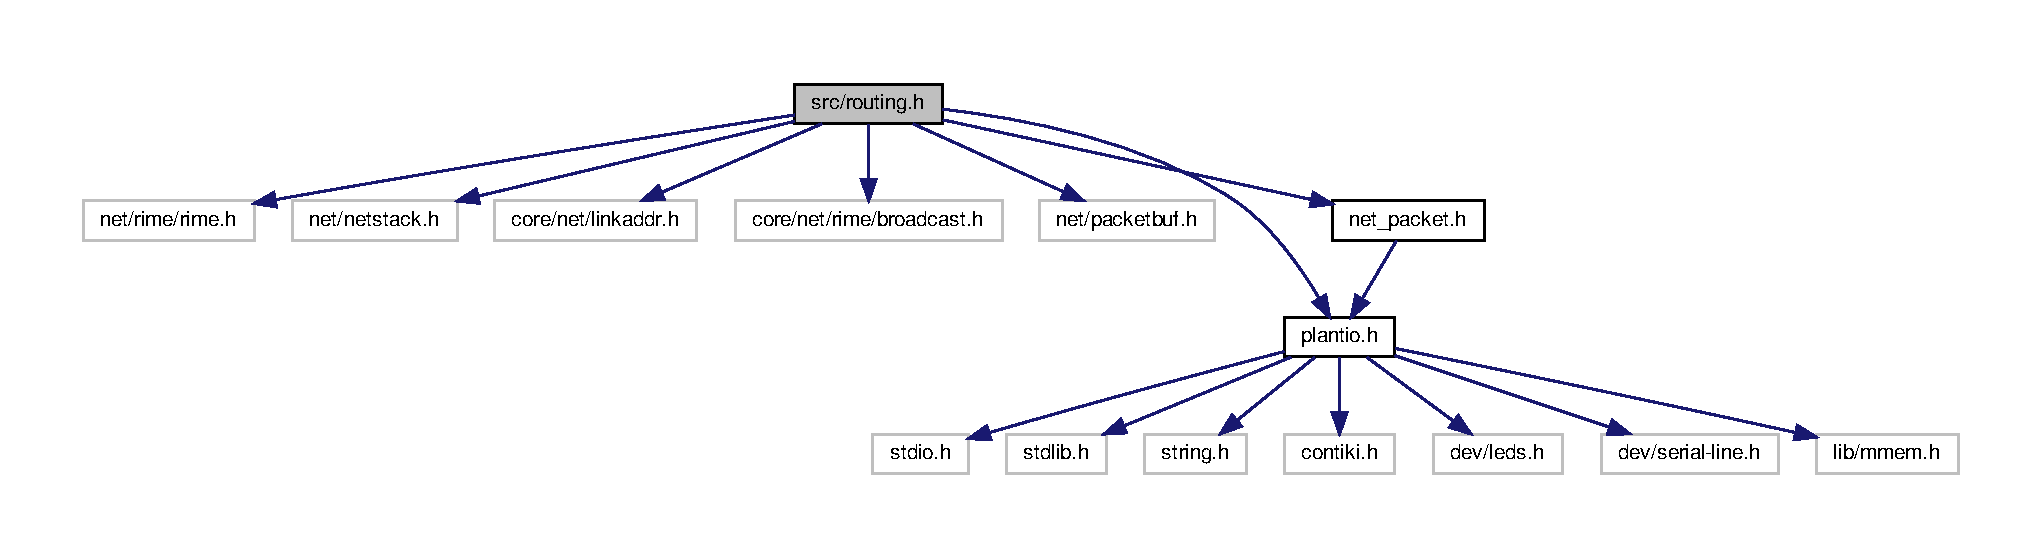
\includegraphics[width=350pt]{routing_8h__incl}
\end{center}
\end{figure}
This graph shows which files directly or indirectly include this file\+:
\nopagebreak
\begin{figure}[H]
\begin{center}
\leavevmode
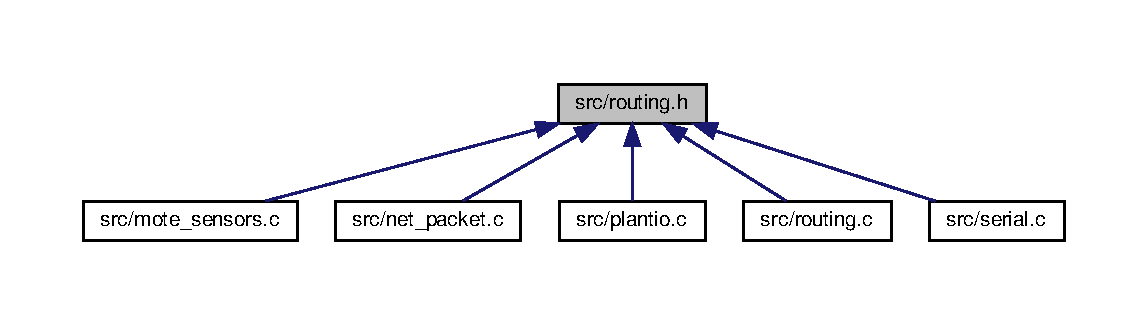
\includegraphics[width=350pt]{routing_8h__dep__incl}
\end{center}
\end{figure}
\subsection*{Functions}
\begin{DoxyCompactItemize}
\item 
void \hyperlink{routing_8h_a13eb496f6046eac861006b61d60dc196}{broadcast\+\_\+receive} (struct broadcast\+\_\+conn $\ast$broadcast, const linkaddr\+\_\+t $\ast$from)
\begin{DoxyCompactList}\small\item\em Callback function for Broadcast. \end{DoxyCompactList}\item 
void \hyperlink{routing_8h_a8a3474e4cd76194d0eb2ac744eda8c7c}{unicast\+\_\+receive} (struct unicast\+\_\+conn $\ast$unicast, const linkaddr\+\_\+t $\ast$from)
\begin{DoxyCompactList}\small\item\em Callback function for Unicast. \end{DoxyCompactList}\item 
void \hyperlink{routing_8h_aa8cb8a8be4c104f1b1405ed682f8e191}{init\+\_\+network} (void)
\begin{DoxyCompactList}\small\item\em Starts the network discovery algorithm. \end{DoxyCompactList}\item 
void \hyperlink{routing_8h_a20f9e50ac25cd018884fec58b70b13a5}{forward\+\_\+discover} (const plantio\+\_\+packet\+\_\+t $\ast$packet)
\begin{DoxyCompactList}\small\item\em Forwards the network discovery packet \& updates the routing tables. \end{DoxyCompactList}\item 
\mbox{\Hypertarget{routing_8h_a52613d7923f35868e7e0dd3e7f2e47dc}\label{routing_8h_a52613d7923f35868e7e0dd3e7f2e47dc}} 
void \hyperlink{routing_8h_a52613d7923f35868e7e0dd3e7f2e47dc}{find\+\_\+best\+\_\+route} (void)
\begin{DoxyCompactList}\small\item\em Finds the optimal route in the routing table by minimizing the number of hops. \end{DoxyCompactList}\item 
\mbox{\Hypertarget{routing_8h_a033ff0c93dd6d1991c523d4466992332}\label{routing_8h_a033ff0c93dd6d1991c523d4466992332}} 
void \hyperlink{routing_8h_a033ff0c93dd6d1991c523d4466992332}{print\+\_\+routing\+\_\+table} (void)
\begin{DoxyCompactList}\small\item\em Prints the routing table. \end{DoxyCompactList}\item 
\mbox{\Hypertarget{routing_8h_a6c7443691d2e4c92e28dc8e13f18fb82}\label{routing_8h_a6c7443691d2e4c92e28dc8e13f18fb82}} 
void \hyperlink{routing_8h_a6c7443691d2e4c92e28dc8e13f18fb82}{clear\+\_\+routing\+\_\+table} (void)
\begin{DoxyCompactList}\small\item\em Clears the routing table. \end{DoxyCompactList}\item 
void \hyperlink{routing_8h_a10c2716d53419a0ec9111c644904c9b9}{write\+\_\+routing\+\_\+table} (const uint8\+\_\+t $\ast$route, const uint8\+\_\+t length)
\begin{DoxyCompactList}\small\item\em Write a route to the routing table on the flash memory. \end{DoxyCompactList}\item 
const uint16\+\_\+t \hyperlink{routing_8h_a5b87ed069c6951f8d390154609c487c0}{get\+\_\+num\+\_\+routes} (void)
\begin{DoxyCompactList}\small\item\em Get the number of entries in the routing table. \end{DoxyCompactList}\item 
const int16\+\_\+t \hyperlink{routing_8h_a605aa3d917cc42b30dd2ed242970a195}{get\+\_\+best\+\_\+route\+\_\+index} (void)
\begin{DoxyCompactList}\small\item\em Get the index of the optimal route in the routing table. -\/1 if table is empty or the current node is the G\+UI node. \end{DoxyCompactList}\item 
const uint8\+\_\+t \hyperlink{routing_8h_a4b6ac79ba38213a3f4390d5d3a9fb095}{get\+\_\+num\+\_\+hops} (const uint16\+\_\+t index)
\begin{DoxyCompactList}\small\item\em Get the number of hops for a route with given index in the routing table. \end{DoxyCompactList}\item 
void \hyperlink{routing_8h_a4530e9af1504c8a4cf003a3ad4abf818}{get\+\_\+route} (uint8\+\_\+t $\ast$route, const uint16\+\_\+t num\+\_\+hops, const uint16\+\_\+t index)
\begin{DoxyCompactList}\small\item\em Get the route for given index in the routing table. \end{DoxyCompactList}\item 
\mbox{\Hypertarget{routing_8h_ac41726b09440e72c5cc9dee53fc13aec}\label{routing_8h_ac41726b09440e72c5cc9dee53fc13aec}} 
void \hyperlink{routing_8h_ac41726b09440e72c5cc9dee53fc13aec}{init\+\_\+rreq\+\_\+reply} (const uint16\+\_\+t index)
\begin{DoxyCompactList}\small\item\em Selects the optimal route to the G\+UI node and transmits it to the G\+UI node. \end{DoxyCompactList}\item 
void \hyperlink{routing_8h_a3639eb60506758c56bbc601911a71c64}{forward\+\_\+routing} (const plantio\+\_\+packet\+\_\+t $\ast$packet)
\begin{DoxyCompactList}\small\item\em Updates the Source and Destionation of incoming packets and forwards the packet to the next hop if necessary. \end{DoxyCompactList}\item 
void \hyperlink{routing_8h_a8724d80f3f41082d62dbaad8f6ebeedf}{init\+\_\+data\+\_\+packet} (const uint8\+\_\+t type, const uint8\+\_\+t dest, const uint8\+\_\+t $\ast$data, const uint8\+\_\+t data\+\_\+len, int index)
\begin{DoxyCompactList}\small\item\em Sends a data packet (id $>$= 10) to any node in the network. \end{DoxyCompactList}\item 
void \hyperlink{routing_8h_ab97d23714b07247e89e011908d6fafcc}{add\+\_\+device\+\_\+to\+\_\+network} (void)
\begin{DoxyCompactList}\small\item\em Add the current node to an existing network. \end{DoxyCompactList}\item 
void \hyperlink{routing_8h_a2b3ed1fa69f729b9eaeeae3357ed4648}{send\+\_\+best\+\_\+route} (const uint8\+\_\+t dest)
\begin{DoxyCompactList}\small\item\em Sends the best route of current device to the destination via unicast. \end{DoxyCompactList}\item 
void \hyperlink{routing_8h_a0a32fd3503c9d77a6bfb62a66f3e47e1}{receive\+\_\+route} (const plantio\+\_\+packet\+\_\+t $\ast$packet)
\begin{DoxyCompactList}\small\item\em Saves the route in the routing table, starts a timer and schedules an R\+R\+EP to the G\+UI node with the best route. \end{DoxyCompactList}\item 
void \hyperlink{routing_8h_ac960ae2b0934e5ce84cd3cc822eb69be}{send\+\_\+ack} (const uint8\+\_\+t $\ast$route, const uint8\+\_\+t len)
\begin{DoxyCompactList}\small\item\em Sends an A\+CK Packet via the given route. \end{DoxyCompactList}\end{DoxyCompactItemize}
\subsection*{Variables}
\begin{DoxyCompactItemize}
\item 
\mbox{\Hypertarget{routing_8h_a5a6576fde225bfed1b06f8cf761bcb84}\label{routing_8h_a5a6576fde225bfed1b06f8cf761bcb84}} 
struct process \hyperlink{routing_8h_a5a6576fde225bfed1b06f8cf761bcb84}{p\+\_\+conn}
\begin{DoxyCompactList}\small\item\em Broadcast and Unicast Process. \end{DoxyCompactList}\item 
\mbox{\Hypertarget{routing_8h_a4c12d3f6cf50b4f1de83cb9702365575}\label{routing_8h_a4c12d3f6cf50b4f1de83cb9702365575}} 
struct process \hyperlink{routing_8h_a4c12d3f6cf50b4f1de83cb9702365575}{p\+\_\+init\+\_\+reply\+\_\+timer}
\begin{DoxyCompactList}\small\item\em Process for initializing the route reply timer. \end{DoxyCompactList}\item 
\mbox{\Hypertarget{routing_8h_afb579a8e94495eb93381fac29cfdc26c}\label{routing_8h_afb579a8e94495eb93381fac29cfdc26c}} 
struct broadcast\+\_\+conn {\bfseries plantio\+\_\+broadcast}
\item 
\mbox{\Hypertarget{routing_8h_ac047c8eb2acde34e82f694c420d58843}\label{routing_8h_ac047c8eb2acde34e82f694c420d58843}} 
struct unicast\+\_\+conn {\bfseries plantio\+\_\+unicast}
\end{DoxyCompactItemize}


\subsection{Detailed Description}
\begin{DoxyAuthor}{Author}
Patrick Willner (\href{mailto:patrick.willner@tum.de}{\tt patrick.\+willner@tum.\+de}), Andreas Koliopoulos (\href{mailto:ga96leh@mytum.de}{\tt ga96leh@mytum.\+de}), Alexander Schmaus (\href{mailto:ga96fin@mytum.de}{\tt ga96fin@mytum.\+de}) 
\end{DoxyAuthor}
\begin{DoxyVersion}{Version}
0.\+1 
\end{DoxyVersion}
\begin{DoxyDate}{Date}
2019-\/12-\/12
\end{DoxyDate}
\begin{DoxyCopyright}{Copyright}
Copyright (c) 2019 
\end{DoxyCopyright}


\subsection{Function Documentation}
\mbox{\Hypertarget{routing_8h_ab97d23714b07247e89e011908d6fafcc}\label{routing_8h_ab97d23714b07247e89e011908d6fafcc}} 
\index{routing.\+h@{routing.\+h}!add\+\_\+device\+\_\+to\+\_\+network@{add\+\_\+device\+\_\+to\+\_\+network}}
\index{add\+\_\+device\+\_\+to\+\_\+network@{add\+\_\+device\+\_\+to\+\_\+network}!routing.\+h@{routing.\+h}}
\subsubsection{\texorpdfstring{add\+\_\+device\+\_\+to\+\_\+network()}{add\_device\_to\_network()}}
{\footnotesize\ttfamily void add\+\_\+device\+\_\+to\+\_\+network (\begin{DoxyParamCaption}\item[{void}]{ }\end{DoxyParamCaption})}



Add the current node to an existing network. 

Starts a broadcast to neighbouring nodes which then reply with their best route to the G\+UI node. \mbox{\Hypertarget{routing_8h_a13eb496f6046eac861006b61d60dc196}\label{routing_8h_a13eb496f6046eac861006b61d60dc196}} 
\index{routing.\+h@{routing.\+h}!broadcast\+\_\+receive@{broadcast\+\_\+receive}}
\index{broadcast\+\_\+receive@{broadcast\+\_\+receive}!routing.\+h@{routing.\+h}}
\subsubsection{\texorpdfstring{broadcast\+\_\+receive()}{broadcast\_receive()}}
{\footnotesize\ttfamily void broadcast\+\_\+receive (\begin{DoxyParamCaption}\item[{struct broadcast\+\_\+conn $\ast$}]{broadcast,  }\item[{const linkaddr\+\_\+t $\ast$}]{from }\end{DoxyParamCaption})}



Callback function for Broadcast. 


\begin{DoxyParams}{Parameters}
{\em broadcast} & Broadcast Connection \\
\hline
{\em from} & Node ID of packet source \\
\hline
\end{DoxyParams}
\mbox{\Hypertarget{routing_8h_a20f9e50ac25cd018884fec58b70b13a5}\label{routing_8h_a20f9e50ac25cd018884fec58b70b13a5}} 
\index{routing.\+h@{routing.\+h}!forward\+\_\+discover@{forward\+\_\+discover}}
\index{forward\+\_\+discover@{forward\+\_\+discover}!routing.\+h@{routing.\+h}}
\subsubsection{\texorpdfstring{forward\+\_\+discover()}{forward\_discover()}}
{\footnotesize\ttfamily void forward\+\_\+discover (\begin{DoxyParamCaption}\item[{const plantio\+\_\+packet\+\_\+t $\ast$}]{packet }\end{DoxyParamCaption})}



Forwards the network discovery packet \& updates the routing tables. 

Packets with current Node ID in the source as well as transmissions below P\+L\+A\+N\+T\+I\+O\+\_\+\+M\+I\+N\+\_\+\+R\+S\+SI threshold will be dropped.


\begin{DoxyParams}{Parameters}
{\em packet} & Pointer to instance of plantio\+\_\+packet\+\_\+t \\
\hline
\end{DoxyParams}
\mbox{\Hypertarget{routing_8h_a3639eb60506758c56bbc601911a71c64}\label{routing_8h_a3639eb60506758c56bbc601911a71c64}} 
\index{routing.\+h@{routing.\+h}!forward\+\_\+routing@{forward\+\_\+routing}}
\index{forward\+\_\+routing@{forward\+\_\+routing}!routing.\+h@{routing.\+h}}
\subsubsection{\texorpdfstring{forward\+\_\+routing()}{forward\_routing()}}
{\footnotesize\ttfamily void forward\+\_\+routing (\begin{DoxyParamCaption}\item[{const plantio\+\_\+packet\+\_\+t $\ast$}]{packet }\end{DoxyParamCaption})}



Updates the Source and Destionation of incoming packets and forwards the packet to the next hop if necessary. 


\begin{DoxyParams}{Parameters}
{\em packet} & Instance of packet struct \\
\hline
\end{DoxyParams}
\mbox{\Hypertarget{routing_8h_a605aa3d917cc42b30dd2ed242970a195}\label{routing_8h_a605aa3d917cc42b30dd2ed242970a195}} 
\index{routing.\+h@{routing.\+h}!get\+\_\+best\+\_\+route\+\_\+index@{get\+\_\+best\+\_\+route\+\_\+index}}
\index{get\+\_\+best\+\_\+route\+\_\+index@{get\+\_\+best\+\_\+route\+\_\+index}!routing.\+h@{routing.\+h}}
\subsubsection{\texorpdfstring{get\+\_\+best\+\_\+route\+\_\+index()}{get\_best\_route\_index()}}
{\footnotesize\ttfamily const int16\+\_\+t get\+\_\+best\+\_\+route\+\_\+index (\begin{DoxyParamCaption}\item[{void}]{ }\end{DoxyParamCaption})}



Get the index of the optimal route in the routing table. -\/1 if table is empty or the current node is the G\+UI node. 

\begin{DoxyReturn}{Returns}
const int16\+\_\+t Index of route in the routing table 
\end{DoxyReturn}
\mbox{\Hypertarget{routing_8h_a4b6ac79ba38213a3f4390d5d3a9fb095}\label{routing_8h_a4b6ac79ba38213a3f4390d5d3a9fb095}} 
\index{routing.\+h@{routing.\+h}!get\+\_\+num\+\_\+hops@{get\+\_\+num\+\_\+hops}}
\index{get\+\_\+num\+\_\+hops@{get\+\_\+num\+\_\+hops}!routing.\+h@{routing.\+h}}
\subsubsection{\texorpdfstring{get\+\_\+num\+\_\+hops()}{get\_num\_hops()}}
{\footnotesize\ttfamily const uint8\+\_\+t get\+\_\+num\+\_\+hops (\begin{DoxyParamCaption}\item[{const uint16\+\_\+t}]{index }\end{DoxyParamCaption})}



Get the number of hops for a route with given index in the routing table. 


\begin{DoxyParams}{Parameters}
{\em index} & Index of route in table \\
\hline
\end{DoxyParams}
\begin{DoxyReturn}{Returns}
const uint16\+\_\+t Number of hops 
\end{DoxyReturn}
\mbox{\Hypertarget{routing_8h_a5b87ed069c6951f8d390154609c487c0}\label{routing_8h_a5b87ed069c6951f8d390154609c487c0}} 
\index{routing.\+h@{routing.\+h}!get\+\_\+num\+\_\+routes@{get\+\_\+num\+\_\+routes}}
\index{get\+\_\+num\+\_\+routes@{get\+\_\+num\+\_\+routes}!routing.\+h@{routing.\+h}}
\subsubsection{\texorpdfstring{get\+\_\+num\+\_\+routes()}{get\_num\_routes()}}
{\footnotesize\ttfamily const uint16\+\_\+t get\+\_\+num\+\_\+routes (\begin{DoxyParamCaption}\item[{void}]{ }\end{DoxyParamCaption})}



Get the number of entries in the routing table. 

\begin{DoxyReturn}{Returns}
const uint16\+\_\+t Number of routes 
\end{DoxyReturn}
\mbox{\Hypertarget{routing_8h_a4530e9af1504c8a4cf003a3ad4abf818}\label{routing_8h_a4530e9af1504c8a4cf003a3ad4abf818}} 
\index{routing.\+h@{routing.\+h}!get\+\_\+route@{get\+\_\+route}}
\index{get\+\_\+route@{get\+\_\+route}!routing.\+h@{routing.\+h}}
\subsubsection{\texorpdfstring{get\+\_\+route()}{get\_route()}}
{\footnotesize\ttfamily void get\+\_\+route (\begin{DoxyParamCaption}\item[{uint8\+\_\+t $\ast$}]{route,  }\item[{const uint16\+\_\+t}]{num\+\_\+hops,  }\item[{const uint16\+\_\+t}]{index }\end{DoxyParamCaption})}



Get the route for given index in the routing table. 


\begin{DoxyParams}{Parameters}
{\em route} & Pointer to the allocated memory for the route \\
\hline
{\em num\+\_\+hops} & Number of hops \\
\hline
{\em index} & Index of route in table \\
\hline
\end{DoxyParams}
\mbox{\Hypertarget{routing_8h_a8724d80f3f41082d62dbaad8f6ebeedf}\label{routing_8h_a8724d80f3f41082d62dbaad8f6ebeedf}} 
\index{routing.\+h@{routing.\+h}!init\+\_\+data\+\_\+packet@{init\+\_\+data\+\_\+packet}}
\index{init\+\_\+data\+\_\+packet@{init\+\_\+data\+\_\+packet}!routing.\+h@{routing.\+h}}
\subsubsection{\texorpdfstring{init\+\_\+data\+\_\+packet()}{init\_data\_packet()}}
{\footnotesize\ttfamily void init\+\_\+data\+\_\+packet (\begin{DoxyParamCaption}\item[{const uint8\+\_\+t}]{type,  }\item[{const uint8\+\_\+t}]{dest,  }\item[{const uint8\+\_\+t $\ast$}]{data,  }\item[{const uint8\+\_\+t}]{data\+\_\+len,  }\item[{int}]{index }\end{DoxyParamCaption})}



Sends a data packet (id $>$= 10) to any node in the network. 


\begin{DoxyParams}{Parameters}
{\em type} & Type of packet \\
\hline
{\em dest} & Destination node id \\
\hline
{\em data} & Pointer to byte array data \\
\hline
{\em data\+\_\+len} & Data length \\
\hline
{\em index} & Index of route in table, set to -\/1 if not known \\
\hline
\end{DoxyParams}
\mbox{\Hypertarget{routing_8h_aa8cb8a8be4c104f1b1405ed682f8e191}\label{routing_8h_aa8cb8a8be4c104f1b1405ed682f8e191}} 
\index{routing.\+h@{routing.\+h}!init\+\_\+network@{init\+\_\+network}}
\index{init\+\_\+network@{init\+\_\+network}!routing.\+h@{routing.\+h}}
\subsubsection{\texorpdfstring{init\+\_\+network()}{init\_network()}}
{\footnotesize\ttfamily void init\+\_\+network (\begin{DoxyParamCaption}\item[{void}]{ }\end{DoxyParamCaption})}



Starts the network discovery algorithm. 

Floods the network with a network discory packet. \mbox{\Hypertarget{routing_8h_a0a32fd3503c9d77a6bfb62a66f3e47e1}\label{routing_8h_a0a32fd3503c9d77a6bfb62a66f3e47e1}} 
\index{routing.\+h@{routing.\+h}!receive\+\_\+route@{receive\+\_\+route}}
\index{receive\+\_\+route@{receive\+\_\+route}!routing.\+h@{routing.\+h}}
\subsubsection{\texorpdfstring{receive\+\_\+route()}{receive\_route()}}
{\footnotesize\ttfamily void receive\+\_\+route (\begin{DoxyParamCaption}\item[{const plantio\+\_\+packet\+\_\+t $\ast$}]{packet }\end{DoxyParamCaption})}



Saves the route in the routing table, starts a timer and schedules an R\+R\+EP to the G\+UI node with the best route. 


\begin{DoxyParams}{Parameters}
{\em packet} & Instance of packet struct \\
\hline
\end{DoxyParams}
\mbox{\Hypertarget{routing_8h_ac960ae2b0934e5ce84cd3cc822eb69be}\label{routing_8h_ac960ae2b0934e5ce84cd3cc822eb69be}} 
\index{routing.\+h@{routing.\+h}!send\+\_\+ack@{send\+\_\+ack}}
\index{send\+\_\+ack@{send\+\_\+ack}!routing.\+h@{routing.\+h}}
\subsubsection{\texorpdfstring{send\+\_\+ack()}{send\_ack()}}
{\footnotesize\ttfamily void send\+\_\+ack (\begin{DoxyParamCaption}\item[{const uint8\+\_\+t $\ast$}]{route,  }\item[{const uint8\+\_\+t}]{len }\end{DoxyParamCaption})}



Sends an A\+CK Packet via the given route. 


\begin{DoxyParams}{Parameters}
{\em route} & Path to the destination node \\
\hline
\end{DoxyParams}
\mbox{\Hypertarget{routing_8h_a2b3ed1fa69f729b9eaeeae3357ed4648}\label{routing_8h_a2b3ed1fa69f729b9eaeeae3357ed4648}} 
\index{routing.\+h@{routing.\+h}!send\+\_\+best\+\_\+route@{send\+\_\+best\+\_\+route}}
\index{send\+\_\+best\+\_\+route@{send\+\_\+best\+\_\+route}!routing.\+h@{routing.\+h}}
\subsubsection{\texorpdfstring{send\+\_\+best\+\_\+route()}{send\_best\_route()}}
{\footnotesize\ttfamily void send\+\_\+best\+\_\+route (\begin{DoxyParamCaption}\item[{const uint8\+\_\+t}]{dest }\end{DoxyParamCaption})}



Sends the best route of current device to the destination via unicast. 


\begin{DoxyParams}{Parameters}
{\em dest} & Node id of destination \\
\hline
\end{DoxyParams}
\mbox{\Hypertarget{routing_8h_a8a3474e4cd76194d0eb2ac744eda8c7c}\label{routing_8h_a8a3474e4cd76194d0eb2ac744eda8c7c}} 
\index{routing.\+h@{routing.\+h}!unicast\+\_\+receive@{unicast\+\_\+receive}}
\index{unicast\+\_\+receive@{unicast\+\_\+receive}!routing.\+h@{routing.\+h}}
\subsubsection{\texorpdfstring{unicast\+\_\+receive()}{unicast\_receive()}}
{\footnotesize\ttfamily void unicast\+\_\+receive (\begin{DoxyParamCaption}\item[{struct unicast\+\_\+conn $\ast$}]{unicast,  }\item[{const linkaddr\+\_\+t $\ast$}]{from }\end{DoxyParamCaption})}



Callback function for Unicast. 


\begin{DoxyParams}{Parameters}
{\em unicast} & Unicast Connection \\
\hline
{\em from} & Node ID of packet source \\
\hline
\end{DoxyParams}
\mbox{\Hypertarget{routing_8h_a10c2716d53419a0ec9111c644904c9b9}\label{routing_8h_a10c2716d53419a0ec9111c644904c9b9}} 
\index{routing.\+h@{routing.\+h}!write\+\_\+routing\+\_\+table@{write\+\_\+routing\+\_\+table}}
\index{write\+\_\+routing\+\_\+table@{write\+\_\+routing\+\_\+table}!routing.\+h@{routing.\+h}}
\subsubsection{\texorpdfstring{write\+\_\+routing\+\_\+table()}{write\_routing\_table()}}
{\footnotesize\ttfamily void write\+\_\+routing\+\_\+table (\begin{DoxyParamCaption}\item[{const uint8\+\_\+t $\ast$}]{route,  }\item[{const uint8\+\_\+t}]{length }\end{DoxyParamCaption})}



Write a route to the routing table on the flash memory. 


\begin{DoxyParams}{Parameters}
{\em route} & Array of Node I\+Ds \\
\hline
{\em length} & Length of the array, i.\+e. the number of hops of the route \\
\hline
\end{DoxyParams}

\hypertarget{serial_8c}{}\section{src/serial.c File Reference}
\label{serial_8c}\index{src/serial.\+c@{src/serial.\+c}}
{\ttfamily \#include \char`\"{}serial.\+h\char`\"{}}\newline
{\ttfamily \#include \char`\"{}routing.\+h\char`\"{}}\newline
{\ttfamily \#include \char`\"{}net\+\_\+packet.\+h\char`\"{}}\newline
{\ttfamily \#include \char`\"{}mote\+\_\+sensors.\+h\char`\"{}}\newline
Include dependency graph for serial.\+c\+:\nopagebreak
\begin{figure}[H]
\begin{center}
\leavevmode
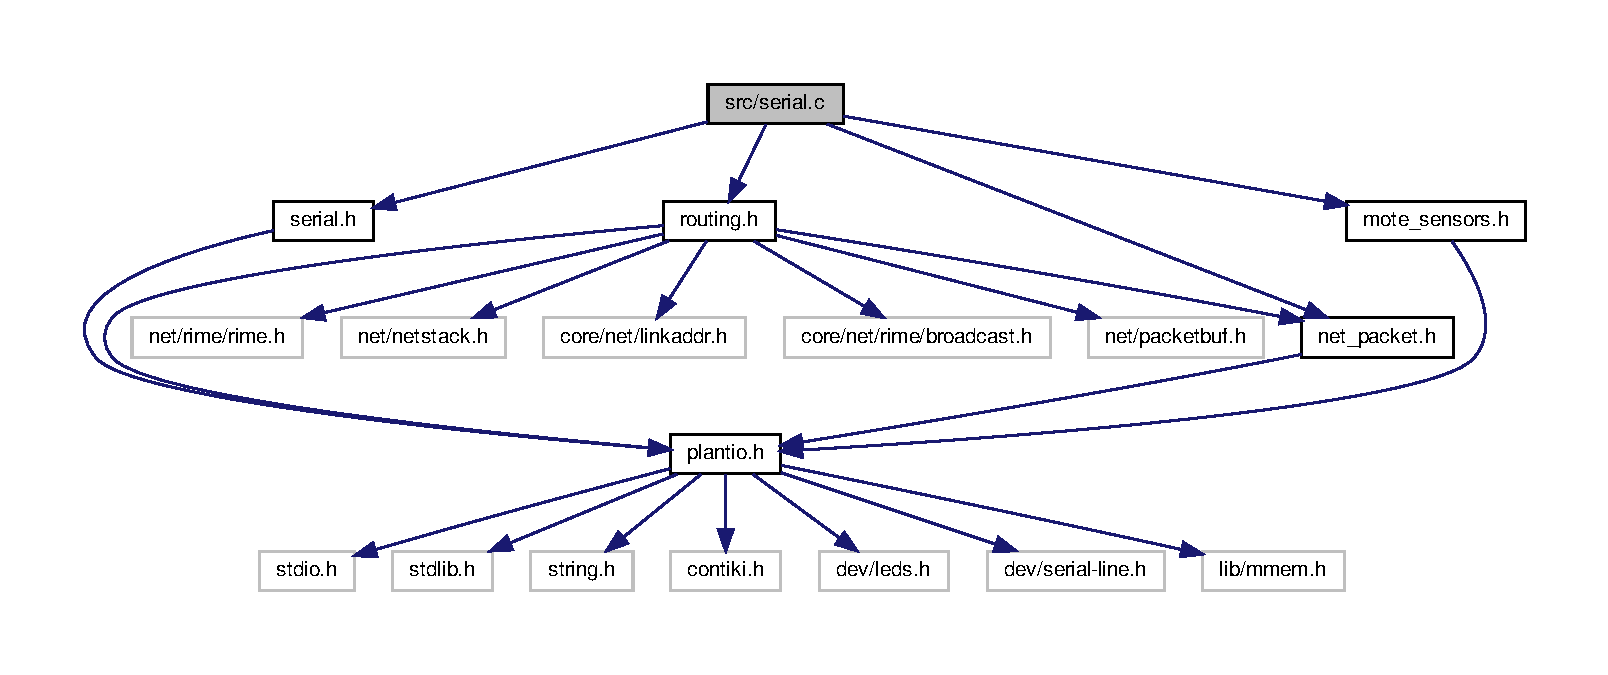
\includegraphics[width=350pt]{serial_8c__incl}
\end{center}
\end{figure}
\subsection*{Functions}
\begin{DoxyCompactItemize}
\item 
\mbox{\Hypertarget{serial_8c_a48d0042e1d3fa2b807e080b401810e07}\label{serial_8c_a48d0042e1d3fa2b807e080b401810e07}} 
{\bfseries P\+R\+O\+C\+E\+SS} (\hyperlink{serial_8h_a93743c0ec4d5fa28a2c26aa266e6f136}{p\+\_\+serial}, \char`\"{}Serial Event listener\char`\"{})
\item 
\mbox{\Hypertarget{serial_8c_a1487fec39db3c42e0079d83a39355737}\label{serial_8c_a1487fec39db3c42e0079d83a39355737}} 
{\bfseries P\+R\+O\+C\+E\+S\+S\+\_\+\+T\+H\+R\+E\+AD} (\hyperlink{serial_8h_a93743c0ec4d5fa28a2c26aa266e6f136}{p\+\_\+serial}, ev, data)
\item 
void \hyperlink{serial_8c_a48f67010ee11dabaea0feb51f2a6ecd3}{parse\+\_\+serial\+\_\+input} (char $\ast$input)
\begin{DoxyCompactList}\small\item\em Parse a serial input char array. \end{DoxyCompactList}\end{DoxyCompactItemize}


\subsection{Detailed Description}
\begin{DoxyAuthor}{Author}
Patrick Willner (\href{mailto:patrick.willner@tum.de}{\tt patrick.\+willner@tum.\+de}), Andreas Koliopoulos (\href{mailto:ga96leh@mytum.de}{\tt ga96leh@mytum.\+de}), Alexander Schmaus (\href{mailto:ga96fin@mytum.de}{\tt ga96fin@mytum.\+de}) 
\end{DoxyAuthor}
\begin{DoxyVersion}{Version}
0.\+1 
\end{DoxyVersion}
\begin{DoxyDate}{Date}
2019-\/12-\/14
\end{DoxyDate}
\begin{DoxyCopyright}{Copyright}
Copyright (c) 2019 
\end{DoxyCopyright}


\subsection{Function Documentation}
\mbox{\Hypertarget{serial_8c_a48f67010ee11dabaea0feb51f2a6ecd3}\label{serial_8c_a48f67010ee11dabaea0feb51f2a6ecd3}} 
\index{serial.\+c@{serial.\+c}!parse\+\_\+serial\+\_\+input@{parse\+\_\+serial\+\_\+input}}
\index{parse\+\_\+serial\+\_\+input@{parse\+\_\+serial\+\_\+input}!serial.\+c@{serial.\+c}}
\subsubsection{\texorpdfstring{parse\+\_\+serial\+\_\+input()}{parse\_serial\_input()}}
{\footnotesize\ttfamily void parse\+\_\+serial\+\_\+input (\begin{DoxyParamCaption}\item[{char $\ast$}]{input }\end{DoxyParamCaption})}



Parse a serial input char array. 

Parse serial input events, received from the G\+UI.


\begin{DoxyParams}{Parameters}
{\em input} & \\
\hline
\end{DoxyParams}

\hypertarget{serial_8h}{}\section{src/serial.h File Reference}
\label{serial_8h}\index{src/serial.\+h@{src/serial.\+h}}


Defines the serial communication between a node and the G\+UI.  


{\ttfamily \#include \char`\"{}plantio.\+h\char`\"{}}\newline
Include dependency graph for serial.\+h\+:
\nopagebreak
\begin{figure}[H]
\begin{center}
\leavevmode
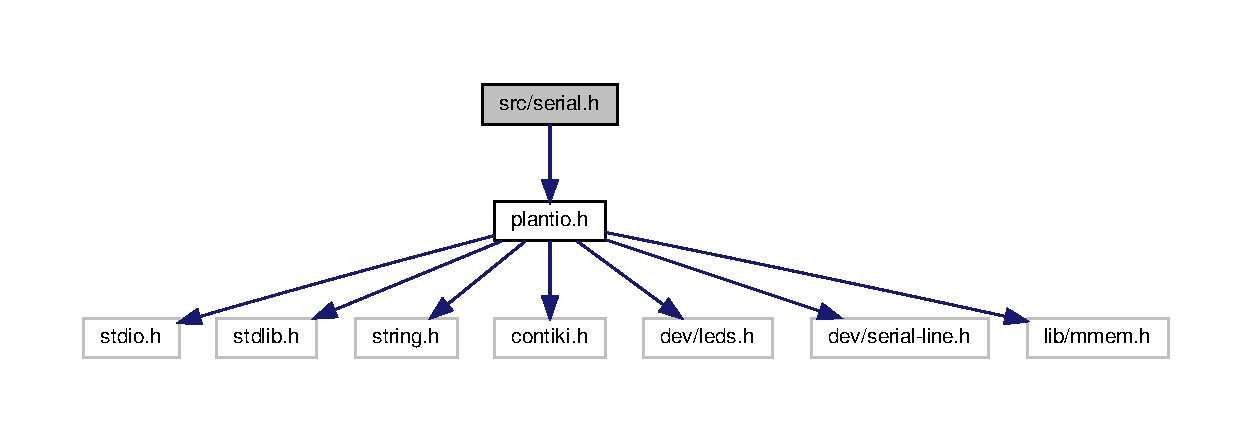
\includegraphics[width=350pt]{serial_8h__incl}
\end{center}
\end{figure}
This graph shows which files directly or indirectly include this file\+:
\nopagebreak
\begin{figure}[H]
\begin{center}
\leavevmode
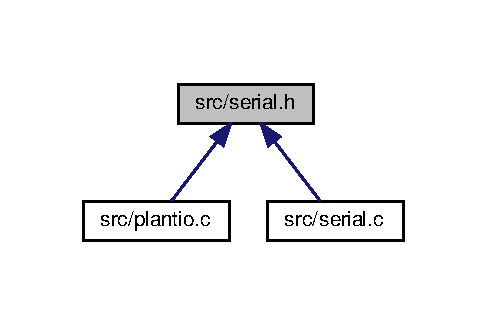
\includegraphics[width=234pt]{serial_8h__dep__incl}
\end{center}
\end{figure}
\subsection*{Functions}
\begin{DoxyCompactItemize}
\item 
void \hyperlink{serial_8h_a48f67010ee11dabaea0feb51f2a6ecd3}{parse\+\_\+serial\+\_\+input} (char $\ast$input)
\begin{DoxyCompactList}\small\item\em Parse serial input events, received from the G\+UI. \end{DoxyCompactList}\end{DoxyCompactItemize}
\subsection*{Variables}
\begin{DoxyCompactItemize}
\item 
\mbox{\Hypertarget{serial_8h_a93743c0ec4d5fa28a2c26aa266e6f136}\label{serial_8h_a93743c0ec4d5fa28a2c26aa266e6f136}} 
struct process \hyperlink{serial_8h_a93743c0ec4d5fa28a2c26aa266e6f136}{p\+\_\+serial}
\begin{DoxyCompactList}\small\item\em Process for handling serial input. \end{DoxyCompactList}\end{DoxyCompactItemize}


\subsection{Detailed Description}
Defines the serial communication between a node and the G\+UI. 

\begin{DoxyAuthor}{Author}
Patrick Willner (\href{mailto:patrick.willner@tum.de}{\tt patrick.\+willner@tum.\+de}), Andreas Koliopoulos (\href{mailto:ga96leh@mytum.de}{\tt ga96leh@mytum.\+de}), Alexander Schmaus (\href{mailto:ga96fin@mytum.de}{\tt ga96fin@mytum.\+de}) 
\end{DoxyAuthor}
\begin{DoxyVersion}{Version}
0.\+1 
\end{DoxyVersion}
\begin{DoxyDate}{Date}
2019-\/12-\/14
\end{DoxyDate}
The following Node to G\+UI strings are defined\+:

Output String (from mote) Description

$<$\$src\+\_\+id\+:route\+:\$r\+\_\+1\+:\$\+\_\+2\+:...$>$ get optimal path to node with id \$src\+\_\+id

$<$\$src\+\_\+id\+:th\+:\$temp\+\_\+low\+:\$temp\+\_\+high\+:\$hum\+\_\+low\+:\$hum\+\_\+high\+:\$light\+\_\+low\+:\$light\+\_\+high$>$ get thresholds of node with id \$src\+\_\+id

$<$\$src\+\_\+id\+:sensor\+\_\+data\+:\$temp\+\_\+1\+:...\+:\$temp\+\_\+2\+:\$hum\+\_\+1\+:...\+:\$hum\+\_\+max\+:\$light\+\_\+1\+:...\+:\$light\+\_\+max$>$get sensors data (temp, hum, light) of node with id \$src\+\_\+id with datapoints 1 to max

$<$\begin{DoxyParagraph}{src\+\_\+id}
t\+:
\end{DoxyParagraph}
data$>$ get routing table of node with id \$src\+\_\+id with \$data formatted equivalent to file structure

$<$\begin{DoxyParagraph}{src\+\_\+id}
ck$>$ acknowledgement for received datapacket from node with id 
\end{DoxyParagraph}
src\+\_\+id

The following G\+UI to Node strings are defined\+:

Input String (from G\+UI) Description

0\+:init Start network discovery from current node

\begin{DoxyParagraph}{dest\+\_\+id}
ed\+:
\end{DoxyParagraph}
args Set L\+ED of node \$dest\+\_\+id, where \$args = \{4\+: blue, 2\+: green, 1\+: red, 7\+: all, ...R\+GB Addition\}

\begin{DoxyParagraph}{dest\+\_\+id}
t Fetch routing table of node 
\end{DoxyParagraph}
dest\+\_\+id

\begin{DoxyParagraph}{dest\+\_\+id}
et\+\_\+th Fetch thresholds of node 
\end{DoxyParagraph}
dest\+\_\+id

\$dest\+\_\+id\+:set\+\_\+th\+:\$temp\+\_\+low\+:\$temp\+\_\+high\+:\$hum\+\_\+low\+:\$hum\+\_\+high\+:\$light\+\_\+low\+:\$light\+\_\+high Set thresholds of node \$dest\+\_\+id

\$dest\+\_\+id\+:get\+\_\+data Get M\+A\+X\+\_\+\+N\+U\+M\+\_\+\+O\+F\+\_\+\+V\+A\+L\+U\+ES values of sensor data (temp, hum, light)

\begin{DoxyCopyright}{Copyright}
Copyright (c) 2019 
\end{DoxyCopyright}


\subsection{Function Documentation}
\mbox{\Hypertarget{serial_8h_a48f67010ee11dabaea0feb51f2a6ecd3}\label{serial_8h_a48f67010ee11dabaea0feb51f2a6ecd3}} 
\index{serial.\+h@{serial.\+h}!parse\+\_\+serial\+\_\+input@{parse\+\_\+serial\+\_\+input}}
\index{parse\+\_\+serial\+\_\+input@{parse\+\_\+serial\+\_\+input}!serial.\+h@{serial.\+h}}
\subsubsection{\texorpdfstring{parse\+\_\+serial\+\_\+input()}{parse\_serial\_input()}}
{\footnotesize\ttfamily void parse\+\_\+serial\+\_\+input (\begin{DoxyParamCaption}\item[{char $\ast$}]{input }\end{DoxyParamCaption})}



Parse serial input events, received from the G\+UI. 


\begin{DoxyParams}{Parameters}
{\em input} & \\
\hline
\end{DoxyParams}
Parse serial input events, received from the G\+UI.


\begin{DoxyParams}{Parameters}
{\em input} & \\
\hline
\end{DoxyParams}

%--- End generated contents ---

% Index
\backmatter
\newpage
\phantomsection
\clearemptydoublepage
\addcontentsline{toc}{chapter}{Index}
\printindex

\end{document}
